%\newif \ifdraft \drafttrue
\newif \ifdraft \draftfalse

\documentclass[10pt]{sigplanconf}
\usepackage[hyphens]{url}
\usepackage{amssymb}
\usepackage{color}
\usepackage{amsthm}
\usepackage{amsmath}
\usepackage{bigstrut}
%\usepackage{alg}
\usepackage[nointegrals]{wasysym}
\usepackage{graphicx}
\usepackage{balance}
\usepackage[override]{cmtt}
\usepackage{algorithm}
\usepackage[noend]{algorithmic}

\ifdraft
\usepackage{color}
\newcommand{\todo}[1]{\textbf{#1}}
\definecolor{purple}{rgb}{0.8,0,0.8}
\newcommand{\sbmcomment}[1]{\textcolor{purple}{SBM -- #1}}
\newcommand{\mwh}[1]{\textcolor{purple}{MWH -- #1}}
\newcommand{\pxm}[1]{\textcolor{red}{PM -- #1}}
\newcommand{\ms}[1]{\textcolor{yellow}{MS -- #1}}
\newcommand{\jnote}[1]{\textcolor{blue}{{\bf JK} -- \emph{#1}}}
\else
\newcommand{\todo}[1]{}
\newcommand{\sbmcomment}[1]{}
\newcommand{\mwh}[1]{}
\newcommand{\pxm}[1]{}
\newcommand{\ms}[1]{}
\newcommand{\jnote}[1]{}
\fi

\conferenceinfo{PLAS'12}{June 15, Beijing, China.}
\copyrightyear{2012}
\copyrightdata{ISBN 978-1-4503-1441-1/12/06}

%%% names
\newcommand{\flowcheck}{\textsc{FlowCheck}}
\newcommand{\parma}{PARMA}

\makeatletter
\newtheorem*{rep@theorem}{\rep@title}
\newcommand{\newreptheorem}[2]{%
\newenvironment{rep#1}[1]{%
 \def\rep@title{#2 \ref{##1}}%
 \begin{rep@theorem}}%
 {\end{rep@theorem}}}
\makeatother

\theoremstyle{plain} % bold head, italicized body  (the default)
\newtheorem{theorem}{Theorem}
\newreptheorem{theorem}{Theorem}
\newtheorem{lemma}[theorem]{Lemma}
\newreptheorem{lemma}{Lemma}
\newtheorem{proposition}[theorem]{Proposition}
\newtheorem{corollary}[theorem]{Corollary}
\newtheorem{axiom}{Axiom}

\newcounter{subtheorem}[theorem]
\newtheorem{subtheorem}[subtheorem]{}
\renewcommand{\thesubtheorem}{\thetheorem{} (\roman{subtheorem})}

% https://secure.wikimedia.org/wikibooks/en/wiki/LaTeX/Theorems
% Fix latex
\def\smallskip{\vskip\smallskipamount}
\def\medskip{\vskip\medskipamount}
\def\bigskip{\vskip\bigskipamount}
 
% Hand made theorem
\def\subtheorem{%
\par\smallskip\indent\refstepcounter{subtheorem}\hbox{\bf%
    (\roman{subtheorem})}%
\it\ %\ignorespaces
}
\def\endsubtheorem{\par\smallskip}
\newenvironment{thm}{\subtheorem}{\endsubtheorem}

\def\subproof#1{%
\par\smallskip\noindent\hbox{{\em} \bf%
    #1.}%
\ %\ignorespaces
}
\def\endsubproof{\qed\par\smallskip}
\newenvironment{subproofe}{\subproof}{\endsubproof}



\theoremstyle{definition} % bold head, normal body
\newtheorem{definition}[theorem]{Definition}
\newtheorem*{definition-un}{Definition}
\newtheorem{notation}[theorem]{Notation}
\newtheorem*{notation-un}{Notation}
\newtheorem{remark}[theorem]{Remark}
\newtheorem*{remark-un}{Remark}
\newtheorem*{claim}{Claim}

\theoremstyle{remark} % italic head, normal body
\newtheorem{example}[theorem]{Example}
\newtheorem*{example-un}{Example}
\newtheorem{examples}[theorem]{Examples}
\newtheorem*{examples-un}{Examples}
\newtheorem*{hint}{Hint}

\newcommand{\imp}{\Rightarrow}
\newcommand{\ybox}[1]{\parbox{5.5in}{\vspace{0.1in} \hl{#1} \vspace{0.1in}}}
\newcommand{\note}[1]{{\textbf{Note: #1}}}
% \newcommand{\todo}[1]{{\color{red}{\textbf{To do:} #1}}}
% \newcommand{\goal}[1]{\ybox{\textbf{Goal}: #1}}
% \newcommand{\activity}[1]{\ybox{\textbf{Research activity}: #1}}
% \newcommand{\problem}[1]{\ybox{\textbf{Research problem}: #1}}
% \newcommand{\question}[1]{\ybox{\textbf{Question}: #1}}

\newcommand{\stacklabel}[1]{\stackrel{\smash{\scriptscriptstyle \mathrm{#1}}}}
\newcommand{\defeq}{\stacklabel{def}=}
\newcommand{\nzset}[1]{\textit{support}(#1)}
\newcommand{\support}[1]{\nzset{#1}}
\newcommand{\overlap}[2]{\textit{overlap}(#1,#2)}
\newcommand{\cp}{\mathbb{C}}
% deleted \ppbot, use \ppzero instead
\newcommand{\pconcfun}{\gamma_{\cp}}
\newcommand{\pconc}[1]{\gamma_{\cp}(#1)}
\newcommand{\psconc}[1]{\gamma_{\powersetb{}{\cp}}(#1)}
\newcommand{\ppconcfun}{\gamma_{\ppolys}}
\newcommand{\ppsconcfun}{\gamma_{\ppowers}}
\newcommand{\ppconc}[1]{\ppconcfun(#1)}
\newcommand{\ppowers}[0]{\powersetb{n}{\ppolys}}
\newcommand{\ppsconc}[1]{\ppsconcfun(#1)}

\newcommand{\abst}[1]{\alpha(#1)}
\newcommand{\lub}[1]{\textit{lub}(#1)}
\newcommand{\glb}[1]{\textit{glb}(#1)}
\newcommand{\chull}[1]{\textit{chull}(#1)}
\newcommand{\dom}[1]{\textit{domain}(#1)}
\newcommand{\fv}[1]{\textit{fv}(#1)}

\newcommand{\var}[1]{\ensuremath{\mathit{#1}}}
\newcommand{\aif}[0]{\text{ \textbf{if} }}
\newcommand{\aendif}[0]{\text{ \textbf{endif} }}
\newcommand{\apif}[0]{\text{ \textbf{pif} }}
\newcommand{\athen}[0]{\text{ \textbf{then} }}
\newcommand{\aelse}[0]{\text{ \textbf{else} }}
\newcommand{\aendpif}[0]{\text{ \textbf{endpif} }}
\newcommand{\atrue}[0]{\text{ \textbf{true} }}
\newcommand{\afalse}[0]{\text{ \textbf{false} }}
\newcommand{\aor}[0]{\text{ \textbf{or} }}
\newcommand{\aand}[0]{\text{ \textbf{and} }}
\newcommand{\asemi}[0]{\text{ \textbf{;} }}
\newcommand{\aassign}[0]{\text{ \textbf{=} }}
\newcommand{\askip}[0]{\text{ \textbf{skip} }}
\newcommand{\aneg}[1]{\neg #1}

\newcommand{\sconst}[1]{\ensuremath{\mathsf{#1}}}
\newcommand{\strue}{\sconst{True}}
\newcommand{\sfalse}{\sconst{False}}
\newcommand{\sskip}{\mathsf{skip}}
\newcommand{\sifk}{\mathsf{if}}
\newcommand{\spifk}{\mathsf{pif}}
\newcommand{\sthenk}{\mathsf{then}}
\newcommand{\selsek}{\mathsf{else}}
\newcommand{\sif}[3]{\sifk\;{#1}\;\sthenk\;{#2}\;\mathsf{else}\;{#3}}
\newcommand{\sifnoelse}[2]{\sifk\;{#1}\;\sthenk\;{#2}}
\newcommand{\spif}[3]{\spifk\;{#1}\;\sthenk\;{#2}\;\mathsf{else}\;{#3}}
\newcommand{\spifnoelse}[2]{\spifk\;{#1}\;\sthenk\;{#2}}
\newcommand{\sassign}[2]{{#1}\;:=\;{#2}}
\newcommand{\sseq}[2]{{#1} \;;\; {#2}}
\newcommand{\swhile}[2]{\mathsf{while}\;{#1}\;\mathsf{do}\;{#2}}
\newcommand{\suniformname}[0]{\mathsf{uniform}}
\newcommand{\suniform}[3]{\suniformname\;{#1}\;{#2}\;#3}
\newcommand{\ebinop}[3]{#2 #1 #3}
\newcommand{\ssecretk}{\mathsf{secret}}
\newcommand{\sbeliefk}{\mathsf{belief}}
\newcommand{\squerydefk}{\mathsf{querydef}}
\newcommand{\squeryk}{\mathsf{query}}

\newcommand{\stmt}{\mathit{S}}
\newcommand{\aexp}{\mathit{E}}
\newcommand{\bexp}{\mathit{B}}
\newcommand{\relop}{\mathit{relop}}
\newcommand{\arithop}{\mathit{aop}}
\newcommand{\aop}[2]{#1\;\arithop\;#2}
\newcommand{\bop}[2]{#1 \;\relop\; #2}

\newcommand{\vars}[0]{\textbf{Var}}
\newcommand{\states}[0]{\textbf{State}}
\newcommand{\dists}[0]{\textbf{Dist}}
\newcommand{\vals}[0]{\textbf{Val}}
\newcommand{\pmass}[1]{\mathord{\parallel}#1\mathord{\parallel}}
\newcommand{\normal}[1]{\text{normal}(#1)}

\newcommand{\sem}[2]{[\![{#1}]\!]{#2}}
\newcommand{\eeval}[2]{[\![{#1}]\!]{#2}}
\newcommand{\eval}[2]{[\![{#1}]\!]{#2}}
\newcommand{\evalp}[2]{[\![{#1}]\!]{#2}}
\newcommand{\pevalp}[2]{[\![{#1}]\!]{#2}}

\newcommand{\ssplit}[1]{\text{ssplit}\paren{#1}}

\newcommand{\sor}[0]{\;|\;}

\newcommand{\polypoint}[1]{\hat{#1}}

\newcommand{\absbexp}[1]{a(#1)}
\newcommand{\absdbexp}[2]{a^{#1}(#2)}

\newcommand{\auniform}[0]{\text{ \textbf{uniform} }}

\newcommand{\repart}[1]{repart\paren{#1}}

\newcommand{\vkill}{\vspace{-10pt plus 5pt minus 5pt}}

%%% groupings
\newcommand{\ceil}[1]{\lceil #1 \rceil}
\newcommand{\floor}[1]{\lfloor #1 \rfloor}
\newcommand{\paren}[1]{\left( #1 \right)}
\newcommand{\bparen}[1]{\left[ #1 \right]}
\newcommand{\aparen}[1]{\langle #1 \rangle}
\newcommand{\tparen}[1]{\bigl( #1 \bigr)}
\newcommand{\sparen}[1]{\left\{ #1 \right\}}
\newcommand{\maxparen}[1]{\max\sparen{#1}}
\newcommand{\minparen}[1]{\min\sparen{#1}}

%%% logic
\newcommand{\lequiv}[0]{\vdash \dashv}
\newcommand{\limp}{\Rightarrow}
\newcommand{\lh}[1]{lh\paren{#1}}
\newcommand{\lps}[1]{p_l\left[#1\right]}
\newcommand{\rps}[1]{p_r\left[#1\right]}
\newcommand{\ass}[1]{h\paren{#1}}
\newcommand{\assb}[1]{\bar{h}\paren{#1}}
\newcommand{\ra}{\rightarrow}
\newcommand{\lra}{\leftrightarrow}
\newcommand{\sA}{\mathfrak{A}}
\newcommand{\sAA}{\mathfrak{A}_A}
\newcommand{\sB}{\mathfrak{B}}
\newcommand{\sBB}{\mathfrak{B}_B}
\newcommand{\sC}{\mathfrak{C}}
\newcommand{\sCC}{\mathfrak{C}_C}
\newcommand{\sD}{\mathfrak{D}}
\newcommand{\sDD}{\mathfrak{D}_D}
\newcommand{\sN}{\mathfrak{N}}
\newcommand{\sNN}{\mathfrak{N}_N}
\newcommand{\Cn}[1]{Cn\paren{#1}}
\newcommand{\Th}[1]{Th\paren{#1}}
\newcommand{\sents}[0]{Sn_L}
\newcommand{\forms}[0]{Fm_L}

\newcommand{\lsep}[0]{. \;}
\newcommand{\qsep}[0]{\; . \;}

%%% number sets
\newcommand{\Natural}{\mathbb{N}}
\newcommand{\Integer}{\mathbb{Z}}
\newcommand{\Rational}{\mathbb{Q}}
\newcommand{\Real}{\mathbb{R}}
\newcommand{\Complex}{\mathbb{C}}

%%% misc
\newcommand{\logtwo}[1]{\lg \left( #1 \right)}
\newcommand{\abs}[1]{\left| #1 \right|}

%%% referencing
\newcommand{\aref}[1]{Axiom \ref{#1}}
\newcommand{\alref}[1]{Algorithm \ref{#1}}
\newcommand{\apref}[1]{Appendix \ref{#1}}
\newcommand{\pref}[1]{Proposition \ref{#1}}
\newcommand{\eref}[1]{Example \ref{#1}}
\newcommand{\fref}[1]{Figure \ref{#1}}
\newcommand{\sref}[1]{Section \ref{#1}}
\newcommand{\rref}[1]{Remark \ref{#1}}
\newcommand{\dref}[1]{Definition \ref{#1}}
\newcommand{\tref}[1]{Theorem \ref{#1}}
\newcommand{\lref}[1]{Lemma \ref{#1}}
\newcommand{\cref}[1]{Condition \cnumref{#1}}
\newcommand{\cnumref}[1]{(\ref{#1})}
\newcommand{\clref}[1]{Claim \cnumref{#1}}


%%% sets
\newcommand{\powerset}[1]{\mathcal{P}\paren{#1}}
\newcommand{\powersetb}[2]{\mathcal{P}_{#1}\paren{#2}}
\newcommand{\set}[1]{\left\{ #1 \right\}}
\newcommand{\setsize}[1]{\left| #1 \right|}
\newcommand{\vect}[1]{\langle #1 \rangle}
\newcommand{\irange}[2]{\set{#1, ..., #2}}
\newcommand{\ssupset}[1]{#1^{+}}
\newcommand{\ssubset}[1]{#1^{-}}

%%% probabilities and moments
\newcommand{\Prob}[1]{\textbf{Pr}\left[#1\right]}
\newcommand{\Expect}[1]{E \left[ #1 \right]}
\newcommand{\Var}[1]{Var \left[ #1 \right]}
\newcommand{\Covar}[2]{Cov \left[ #1, #2 \right]}
\newcommand{\given}{\;|\;}

%%% operations on distributions
\newcommand{\dcond}[2]{#1 | #2}
\newcommand{\pmassmax}[1]{\mathord{\parallel}#1\mathord{\parallel}^\text{max}}
\newcommand{\pmassmin}[1]{\mathord{\parallel}#1\mathord{\parallel}^\text{min}}

%%% probabilistic polyhedra
\newcommand{\maxprobof}[2]{\overline{#1}(#2)}

\newcommand{\ppname}{probabilistic polyhedron}
\newcommand{\ppnames}{probabilistic polyhedra}
\newcommand{\ppsname}{\ppname{} set}
\newcommand{\ppsnames}{\ppname{} sets}
%\newcommand{\pcup}{\mathrel{\vcenter{\offinterlineskip\hbox{\scriptsize$\hspace*{0.1ex}\mathord{+}$}\vskip-1ex\hbox{$\sqcup$}}}}
%\newcommand{\pcap}{\sqcap}
\newcommand{\poly}{C}
\newcommand{\cons}{B}
\newcommand{\polyset}{\mathcal{C}}
\newcommand{\ppoly}{P}
\newcommand{\abseeval}[2]{\langle\!\langle{#1}\rangle\!\rangle\,{#2}}
\newcommand{\absecount}[2]{#2 \# #1}
\newcommand{\pmeet}{\sqcap_{\cp}}
\newcommand{\pjoin}{\sqcup_{\cp}}
\newcommand{\dprod}{\times}
\newcommand{\pprod}{\times}
\newcommand{\pord}{\sqsubseteq_{\cp}}
\newcommand{\pleq}{\sqsubseteq_{\cp}}
\newcommand{\ple}{\sqsubset_{\cp}}
\newcommand{\ppord}{\sqsubseteq_{\ppolys}}
\newcommand{\ppleq}{\ppord}
\newcommand{\pple}{\sqsubset_{\ppolys}}
\newcommand{\distleq}{\leq}
\newcommand{\distle}{\le}
\newcommand{\ppcup}{\mathrel{\tilde{\cup}}}
\newcommand{\ppcap}{\mathrel{\tilde{\cap}}}
\newcommand{\emptypoly}{\emptyset_{\polyset}}
\newcommand{\iszero}[1]{\mathit{iszero}(#1)}
\newcommand{\isempty}[1]{\mathit{isempty}(#1)}
\newcommand{\pa}[0]{\poly_1}
\newcommand{\pb}[0]{\poly_2}
\newcommand{\pc}[0]{\poly_3}
\newcommand{\pp}[1]{P_{#1}}
\newcommand{\distset}[1]{D_{#1}}
\newcommand{\ppeq}[0]{\equiv}
\newcommand{\ppneq}[0]{{\not \equiv}}
\newcommand{\ppzero}[0]{0_{\ppolys}}
\newcommand{\ppfunzero}[0]{\bot_{\ppolys}}
\newcommand{\distzero}[0]{0_{\dists}}
\newcommand{\distfunzero}[0]{\bot_{\dists}}
\newcommand{\pps}[1]{\Delta_{#1}}
\newcommand{\ppsmax}[1]{max_{pp}\paren{#1}}
\newcommand{\ppolys}{\mathbb{P}}
\newcommand{\ppp}[1]{\getpoly{1}}
\newcommand{\ppa}[0]{\pp{1}}
\newcommand{\ppb}[0]{\pp{2}}
\newcommand{\ppc}[0]{\pp{3}}
\newcommand{\pmin}[1]{\mathrm{p}^\mathrm{min}_{#1}}
\newcommand{\pmax}[1]{\mathrm{p}^\mathrm{max}_{#1}}
\newcommand{\smin}[1]{\mathrm{s}^\mathrm{min}_{#1}}
\newcommand{\smax}[1]{\mathrm{s}^\mathrm{max}_{#1}}
\newcommand{\mmin}[1]{\mathrm{m}^\mathrm{min}_{#1}}
\newcommand{\mmax}[1]{\mathrm{m}^\mathrm{max}_{#1}}
\newcommand{\maxh}[1]{\mathrm{h}^\mathrm{max}_{#1}}
\newcommand{\minh}[1]{\mathrm{h}^\mathrm{min}_{#1}}

\newcommand{\vcomp}[0]{\overline{V}}

\newcommand{\parta}[0]{\mathcal{L}}

\newcommand{\ppprob}[2]{#1^{\text{max}}\paren{#2}}
\newcommand{\ppsprob}[2]{#1^{\text{max}}\paren{#2}}

\newcommand{\ppmmin}[1]{\mathrm{M}^\mathrm{min} (#1)}
\newcommand{\ppmmax}[1]{\mathrm{M}^\mathrm{max} (#1)}

\newcommand{\getpoly}[1]{\poly_{#1}}

% assignment
\newcommand{\bassign}[2]{#1 \ra #2}
\newcommand{\stassign}[3]{#1 \bparen{\bassign{#2}{#3}}}
\newcommand{\stsassign}[3]{#1 \bparen{\bassign{#2}{#3}}}
\newcommand{\funassign}[2]{t_{\bassign{#1}{#2}}}
\newcommand{\funinvassign}[2]{t_{\bassign{#1}{#2}}^{-1}}
\newcommand{\eqassign}[3]{\aparen{#1}^{\bassign{#2}{#3}}}
\newcommand{\eqassignsup}[4]{\aparen{#1}^{\bassign{#2}{#3}}_#4}
\newcommand{\dassign}[3]{#1 \bparen{#2 \ra #3}}
\newcommand{\deassign}[3]{#1 \aparen{#2 \ra #3}}

%\newcommand{\pmin}[1]{\lfloor{\ppoly_#1}\rfloor_\mathrm{p}}
%\newcommand{\pmax}[1]{\lceil{\ppoly_#1}\rceil^\mathrm{p}}
%\newcommand{\smin}[1]{\lfloor{\ppoly_#1}\rfloor_\mathrm{s}}
%\newcommand{\smax}[1]{\lceil{\ppoly_#1}\rceil^\mathrm{s}}
%\newcommand{\mmin}[1]{\lfloor{\ppoly_#1}\rfloor_\mathrm{m}}
%\newcommand{\mmax}[1]{\lceil{\ppoly_#1}\rceil^\mathrm{m}}
%\newcommand{\getpoly}[1]{\pentagon{#1}}
\newcommand{\psize}[1]{\#(#1)}
\newcommand{\phull}[1]{hull\paren{#1}}
\newcommand{\pinter}[2]{#1 \cap #2}
\newcommand{\ppplus}{+}
\newcommand{\pessoverlap}[2]{#1 \mathrel{\frownie} #2}
\newcommand{\optoverlap}[2]{#1 \mathrel{\smiley} #2}
\newcommand{\abspevalp}[2]{\langle\!\langle{#1}\rangle\!\rangle\,{#2}}
%\newcommand{\absdcond}[2]{#1 \wr #2}
\newcommand{\absdcond}[2]{#1 \mid #2}
\newcommand{\abspolicy}[3]{\mathit{tsecure}_{#3}(#1,#2)}
\newcommand{\abspolicyname}{\mathit{tsecure}}

\newcommand{\simplify}[2]{\floor{#1}_{#2}}
\newcommand{\bigsimplify}[2]{\Bigl\lfloor{#1}\Bigr\rfloor_{#2}}

%%% semantic sets and meta-variables
\newcommand{\Z}{\Integer}
\newcommand{\ineq}{\beta}

\newcommand{\project}[2]{#1 \upharpoonright #2}
\newcommand{\forget}[2]{\mathrm{f}_{#1}(#2)}
%\newcommand{\newdim}[2]{\mathrm{e}_{#1}(#2)}

\newcommand{\deleted}[1]{}

\newcommand{\pcase}[1]{\textsc{case} {#1}: }

%%% for proofs in appendix
\newcommand{\eqclass}[3]{\bparen{#1}_{#2}^{#3}}
\newcommand{\eqclassc}[3]{\overline{\bparen{#1}}_{#2}^{#3}}

\newcommand{\mathstep}[1]{\text{[ #1 ]}}
\newcommand{\lfp}{\mathrm{lfp}}

\newcommand{\kw}[1]{\mathtt{#1}}
\newcommand{\polc}{\textsf{tcheck}}
\newcommand{\polcall}{\textsf{tcheck\_all}}

\title{Knowledge-Oriented Secure Multiparty Computation}
\authorinfo{Piotr Mardziel, Michael Hicks, \\ Jonathan Katz}
           {University of Maryland, College Park}
           {\{piotrm,mwh,jkatz\}@cs.umd.edu}
\authorinfo{Mudhakar Srivatsa}
           {IBM T.J. Watson Research Laboratory}
           {msrivats@us.ibm.com}
\begin{document}

\maketitle

\begin{abstract}
Protocols for \emph{secure multiparty computation} (SMC) allow a set
of mutually distrusting parties to compute a function~$f$ of their
private inputs while revealing nothing about their inputs beyond what
is implied by the result.  Depending on~$f$, however, the result
itself may reveal more information than parties are comfortable with.
Almost all previous work on SMC treats $f$ as given.  Left unanswered
is the question of how parties should decide whether it is ``safe''
for them to compute $f$ in the first place.

We propose here a way to apply \emph{belief tracking} to~SMC in order
to address exactly this question. In our approach, each participating
party is able to reason about the increase in knowledge that other
parties could gain as a result of computing $f$, and may choose not to
participate (or participate only partially) so as to restrict that
gain in knowledge.  We develop two techniques---the \emph{belief set}
method and the \emph{SMC belief tracking} method---prove them sound,
and discuss their precision/performance tradeoffs using a series of
experiments.
% Our work gives parties the ability to evaluate
% functions over their secret data while enforcing knowledge-based
% policies limiting how much the parties are allowed to infer about each
% others' inputs.
%The techniques of secure computation allow
%potentially mistrusting parties to evaluate a function of their secret
%data revealing nothing but what can be inferred from the output of
%said function. That which can be inferred, however, can often reveal
%much about the protected secrets. The techniques involved in belief
%tracking, on the other hand, model the inference and can be used to
%protect data by evaluating how much about the secret can be inferred
%from the output of a function. Existing methods, however, are only
%able to consider a single party protecting secret data. In this paper
%we describe a marriage of the techniques, having the ability to
%evaluate functions over multiple parties' secret data while enforcing
%a policy limiting how much the participants can infer about each other.
\end{abstract}

\category{D.2.0}{Software Engineering}{Protection Mechanisms}
\terms Security, Language

% keywords:
%  information flow, secure multiparty computation, knowledge based security

\section{Introduction}
Consider a scenario where $N$ parties $P_1, \ldots, P_N$ wish to
compute some (known) function $f(s_1, \ldots, s_N)$ of their
respective inputs, while ensuring \emph{privacy} of their inputs to
the extent possible.  If these parties all trust some entity~$P_T$,
then each party $P_i$ can simply send its input~$s_i$ to this trusted
entity, who can in turn evaluate $f(s_1, \ldots, s_n)$ and return the
result to each party.  In the more general case, where $f$ is a
vector-valued function returning outputs $out_1,\ldots,out_N$, the
trusted entity gives $out_i$ to party~$P_i$.

Cryptographic protocols for \emph{secure multiparty computation}
(SMC)~\cite{Yao86,GMW87} allow the parties to accomplish the same task
without the involvement of any trusted entity.  (The reader can refer
to a recent overview of SMC~\cite{LindellPinkasPPDM}, or a
textbook-level treatment~\cite{Goldreich04}.)  That is, by running a
distributed protocol amongst themselves the parties can learn the
desired result~$f(s_1, \ldots, s_N)$ (or, in the general case, each
party $P_i$ learns the result~$out_i$) while ensuring that no
information about other party's input is revealed beyond what is
implied by the result(s).  Section~\ref{sec:MPC-overview} provides
further details about the precise notion of security that SMC
protocols achieve.
%The details of how such protocols can be constructed are irrelevant
%for the present paper; the definition of what SMC protocols achieve, however, is pertinent and will be discussed
%in further detail in .

Most work on SMC provides an answer to the question of \emph{how} to
compute~$f$, but does not address the complementary question of
\emph{when} it is ``safe'' to compute~$f$ in the first place, i.e.,
when the output of $f$ may reveal more information than parties are
comfortable with.  The two exceptions that we know
of~\cite{EC:DKMMN06,C:BeiNisOmr08} decide $f$'s safety
\emph{independently} of the parties' inputs and in \emph{isolation} of
any (known or assumed) prior knowledge that parties have about each
others' inputs. 

However, the information implied by a query's result depends both on the parties'
inputs and their prior knowledge. As an example of the former, suppose
two parties want to compute the ``less than or equal'' function,
$f(s_1, s_2) \defeq s_1 \leq s_2$ with variables ranging in $ \set{1, \ldots,
  10} $.  This function could reveal a lot about $ s_1 $ to $ P_2
$. If $s_2=1$ and $f(s_1, s_2)$ returns \emph{true}, then $P_2$ learns
that $s_1$ can only be the value $1$. However, if $s_2=5$ then
regardless of the output of the function, $P_2$ only learns that $s_1$
is one of 5 possibilities, a lower level of knowledge than in the
first case.

On the other hand we may deem a pair of queries acceptable in
isolation, but allowing their composition would be too
revealing.  For example, suppose the parties also want to compute
``greater than or equal'', $f_2(s_1,s_2) \defeq s_1 \geq s_2$. When $
s_2 = 5 $, either query in isolation narrows the values of $ s_1 $ to
a set of at least 4 possibilities from $ P_2 $'s perspective. But if $
f_1 $ and $ f_2 $ both return \emph{true}, $ P_2 $ can infer $ s_1 =
s_2 = 5 $.

%On the other hand we may deem a pair of queries acceptable in
%\emph{isolation}, but allowing their composition would be unsafe.  For
%example, suppose three parties want to compute $f_1(s_1,s_2,s_3)
%\defeq (s_1 = s_2) \vee (s_1 = s_3)$ while $f_2(s_1,s_2,s_3) \defeq
%(s_2 = s_1) \vee (s_2 = s_3)$; i.e., $f_1$ is true if $s_1$ is equal
%to either of $s_2$ or $s_3$, while $f_2$ is true if $s_2$ is equal to
%either of $s_1$ or $s_3$.  Then, assuming the $s_i$ are uniformly
%distributed, any output of either $f_1$ or $f_2$ does little to narrow
%the possible values of the $s_i$. But if $f_1$ returns \emph{true} and
%then $f_2$ returns \emph{false}, all parties know that $s_1 = s_3$,
%which means $P_1$ and $P_3$ now know the other's secret exactly.
 
% A trivial example is when $f$ is the identity function. A less trivial
% example
%  % is given by the case
% where $N=2$,
% %  the parties' inputs are viewed as \emph{sets} over some fixed universe~$\mathcal{U}$, and $f$ computes
% % the intersection of the parties' sets. If $P_2$ holds $s_2=\mathcal{U}$, then the output of~$f$ reveals $P_1$'s
% % input entirely.
% % Yet another example, again assuming $N=2$,
% is given by computation of the ``less-than'' function
% Information can also be combined from several executions of SMC; e.g.,
% if the parties first learn that $s_1 \geq s_2$ and later
% learn that $s_1 \leq s_2$, then both parties can deduce that $s_1=s_2$ and hence have learned each others' inputs
% entirely.

% % A few examples illustrate the limitations of any such approach:
% % \begin{itemize}
% % \item Considering the computation of set intersection would result in the conclusion
% % that $f$ is always unsafe to compute. In fact, however, when $P_2$'s input set $s_2$ is sufficiently small
% % (thus preventing the situation described above), then $P_1$ may be willing to reveal the intersection of its own set
% % with~$s_2$.
% % \item
% In the extreme case, many functions would be rejected, such as the less-than function
% above due to the limit case where we could have $s_2 = 2$ and $s_2 = 1$.

In recent work~\cite{mardziel11belief} we developed an approach
to judging query safety called \emph{knowledge-based security
  enforcement}~(KBSE).  In this paper we show how KBSE can be
generalized to SMC to address the limitations of current techniques
listed above.  

KBSE relies on reasoning about other parties' knowledge of one's own
private data in order to determine whether a given function $f$ is
``safe'' to compute in a given instance.  Our previous work was in an
\emph{asymmetric} setting where only one of the parties (say, $P_1$)
was concerned about privacy.  The other parties' inputs could be
revealed publicly, or at the very least be revealed to~$P_1$; as such,
the previous work did not involve SMC at all.  At a high level, and
specializing to the two-party case, party~$P_1$ knows its own
private data~$s_1$ along with $P_2$'s input~$s_2$, and also maintains
a \emph{belief} about $P_2$'s knowledge of~$s_1$ (represented as a
probability distribution $\delta$).  Before agreeing to compute a
function $f(s_1, s_2)$, $P_1$ determines whether computing the
residual function $f(\cdot, s_2)$ would reveal ``too much
information'' as determined according to a threshold $ 0 < t_1 \leq 1
$ set by~$P_1$.  In particular, $P_1$ will not compute the function if
$P_2$'s belief about the likelihood of a possible secret value
(including the actual secret $s_1$) increases above
$t_1$.\footnote{The release criterion considers all possible values
  for $s_1$ --- and not just the actual value of~$s_1$ --- so that a
  refusal to participate does not leak any information about~$s_1$.}
If $P_1$ does reveal $f(s_1,s_2)$ then it determines what $P_2$ will
learn from the output and revises its estimate $\delta_2$ of $P_2$'s
knowledge accordingly.  It will use this new estimate when considering
subsequent functions.  (KBSE is reviewed in
Section~\ref{sec:KBSE-asymmetric}.)

In our prior work, $P_1$'s determination as to whether it should agree
to compute $f$ relied in an essential way on the fact that $P_1$ knows
the input $s_2$ of the other party. In the SMC setting the privacy of
\emph{all} parties' inputs should be preserved, so our prior
techniques cannot be applied directly.
% An additional challenge in the symmetric setting is the requirement
% for each party to perform belief tracking (about all other parties'
% knowledge of their own input), rather than just having a single
% party perform belief tracking.
In this paper we initiate the idea of combining KBSE and SMC, in order
to address the question of when it is safe to compute some
function~$f$ of multiple parties' inputs. 

We present two techniques (Section~\ref{sec:SMC-KBSE}).  The first,
which we call the \emph{belief set} method, works as follows.  Each
$P_i$ maintains an estimate of the \emph{set} of distributions
$\Delta_j$ for each other principal $P_j$, one for each possible
valuation of $s_j$ (assigned probability 1).  In short, $P_j$'s actual
belief $\delta_j$ is a member of the set $\Delta_j$.  The same basic
procedure as in the prior work, lifted from distributions to sets of
distributions, can then be applied by each $P_i$, and if all agree to
participate, they perform the function evaluation via SMC.

The second technique we call \emph{SMC belief tracking}.  
Rather than have each
principal $P_i$ perform the KBSE procedure individually before the SMC
takes place, the KBSE procedure is performed \emph{within the SMC
  itself}.  If the SMC-KBSE procedure determines that any of the
thresholds $t_i$ will be exceeded by sending a response to $P_j$ then
$P_j$ receives a rejection, rather than the actual answer.  However,
because $P_k$'s knowledge will be different, it could receive a proper
answer.  By performing KBSE within the SMC, we can look at the
\emph{actual} secret values of each of the participants and by
accepting/rejecting selectively, we can ensure that no information is
revealed by rejection.  As we show in Section~\ref{sec:evaluation}
using a series of experiments with our proof-of-concept
implementation, SMC belief tracking is strictly more precise (in that
fewer queries will be rejected) than belief sets.  On the other hand,
SMC is known to be very slow, and so implementing KBSE as an SMC could
be quite costly.  We leave exploration of implementation strategies to
future work.

In summary, the main contribution of this paper is a pair of
techniques for evaluating the safety of SMC computations.  To our
knowledge, ours is the first work to consider the question of safety
in the context parties' actual secrets and prior knowledge, and
approach that should allow more queries to be answered safely, even in
composition.

\section{Secure Multiparty Computation}
\label{sec:MPC-overview}

This section presents basic background on secure multiparty
computation (a completely formal treatment of the security provided by
SMC is beyond the scope of this paper).  Throughout this paper we
assume that all parties are \emph{semi-honest}. This means that they
run any specified protocol exactly as prescribed, but may try to
infer information about other parties' inputs based on their
\emph{view} of the protocol execution.
(A party's view consists of its
local state, along with all messages that it sent or received.) We also assume that parties do not collude.
SMC can be extended to malicious parties who behave arbitrarily, as well as to handle
collusion, but these
complicate the treatment and are tangential to our main thrust.

As described in the introduction, we consider a scenario where $N$
mutually distrusting parties $P_1, \ldots, P_N$ wish to compute some
(known) function $f(s_1, \ldots, s_N)$ of their respective inputs,
while ensuring \emph{privacy} of their inputs to the extent possible.
In an ideal scenario, the parties would all have access to a trusted
entity $P_T$ who would compute the function on their behalf. That is,
each party $P_i$ would simply send its input~$s_i$ to~$P_T$, who would
in turn evaluate $(out_1, \ldots, out_n) = f(s_1, \ldots, s_n)$ and
return the result $out_i$ to party~$P_i$. We write $out
= f(...)$ if the same output is sent to all participants.  If $f$ is a
probabilistic function, then $P_T$ evaluates it using uniform random
choices.

Fix some distributed protocol $\Pi$ that computes~$f$. (This just
means that when the parties run the protocol using their inputs $s_1,
\ldots, s_N$, the protocol terminates with each party holding
output~$out_i$.) We say that $\Pi$ is \emph{secure} if it emulates the
ideal computation of~$f$ described above (where a trusted entity is
available). Specifically, an execution of $\Pi$ should reveal no
information beyond what is revealed in the ideal
computation.\footnote{Readers who are familiar with SMC may note that
  this definition is slightly simpler than usual. The reason is that
  we are considering semi-honest security, and in this paragraph
  assume a deterministic function for simplicity. We are also glossing
  over various technical subtleties that are inessential to get the
  main point across.} This is formally defined by requiring that any
party in the ideal world can sample from a distribution that is
``equivalent'' to the distribution of that party's view in a
real-world execution
of~$\Pi$. %, where a party's view consists of its internal state
%plus the messages it sends and receives.
% \jnote{Note: this assumes no collusion between users.}
Since any party $P_i$ in the ideal world knows only its own input $s_i$ and the output~$out_i$ that it received
from~$P_T$, this implies that $\Pi$ achieves the level of privacy desired. We stress that not only is no information
(beyond the output) about any \emph{single} party's input is revealed, but also no \emph{joint} information about
several parties' inputs is revealed either (just as in the ideal world).

The cryptographic literature considers several notions of what it means for two distributions $D, D'$ to be
``equivalent''. The simplest notion is to require $D, D'$ to be \emph{identical}. If this is the case for
the distributions described above, then $\Pi$ is said to achieve \emph{perfect} security. Alternately, we may
require that $D, D'$ be indistinguishable by computationally bounded algorithms. (We omit a formal definition,
though remark that this notion of indistinguishability is pervasive in all of cryptography, beyond~SMC.)
In this case, we say that $\Pi$ achieves \emph{computational} security.
Perfect security is achievable for $N \geq 3$, whereas only computational security is possible for~$N=2$.

In the remainder of the paper we assume that the secrets $s_i$ remains fixed during a sequence of computations, so that information
gained about $s_i$ from one computation carries over to the next.  We also assume that the $P_i$
have no means to communicate outside the SMC, so that what can be learned
about a particular secret depends only on the functions computed via
an SMC.  We leave relaxation of these restrictions to future work.

\section{Knowledge-Based Security Policies}
\label{sec:KBSE-asymmetric}

Our goal is to devise a method whereby each principal can determine
whether participation in an SMC would reveal too much information
about its secret.  In prior work~\cite{mardziel11belief} we developed
a solution for a special case of this problem. In this case we have
two principals, $P_1$ and $P_2$, and only $P_1$ has a secret value
$x_1$.  In this situation, $P_2$
wishes to compute some function $Q$ of $x_1$, and $P_1$ only wishes to
proceed if $P_2$ remains uncertain about $x_1$ upon learning the
result.  If this is the case, $P_1$ computes the result $n$ and sends
it back to $P_2$.  If not, it sends a rejection message.

The key question is: how does $P_1$ reason what $P_2$ might learn
about $x_1$ based on the output of $Q$?  To answer this question, we
adopted the approach of Clarkson et
al.~\cite{clarkson09quantifying}. In their approach, $P_2$ has a
\emph{belief} about the possible values of $x_1$. They show how that
belief can be revised upon learning the output of a function over that
secret.  In our approach, $P_1$ \emph{estimates} what $P_2$ might know
about $x_1$ (e.g., that it is uniformly distributed), and then uses
Clarkson et al.'s method to determine how much information $P_2$ might
gain from the answer to $Q$.  If this information exceeds a threshold,
the query is rejected.

In the remainder of this section, we describe Clarkson
et al's technique, and then our application of it to knowledge-based
security enforcement.  In the next section, we show how this
approach can be generalized to the SMC setting.

\begin{figure}[t]
\[ \begin{array}{llcl}
\mathit{Variables} & x & \in & \vars \\
\mathit{Integers} & n,s,o & \in & \Integer \\
\mathit{Rationals} & r & \in & \Rational \\
\mathit{Arith. ops} & \arithop &::= & + \mid \times \mid - \\
\mathit{Rel. ops} & \relop &::= & \leq \;\mid\; < \;\mid\; = \;\mid\; \neq \;\mid\; \cdots
\\
\mathit{Arith. exps} & \aexp &::= & x \mid n \mid \aop{\aexp_1}{\aexp_2} \\
\mathit{Bool. exps} & \bexp &::= & \bop{\aexp_1}{\aexp_2} \mid \\
% \strue \mid \sfalse \mid \\
& && \bexp_1 \wedge \bexp_2 \mid \bexp_1 \vee \bexp_2 \mid \aneg{\bexp} \\
\mathit{Statements} & Q,\stmt &::= & \sskip \mid \sassign{x}{\aexp} \mid \\
&     && \sif{\bexp}{\stmt_1}{\stmt_2} \mid \\
&     && \spif{r}{\stmt_1}{\stmt_2} \mid \\
&     && \sseq{\stmt_1}{\stmt_2} \mid \swhile{\bexp}{\stmt} % \mid \\
% &     && \suniform{x}{n_1}{n_2} \\
\end{array} \]
\vspace*{-0.1in}
\caption{Core language syntax} \label{fig:syntax}
\vspace*{-0.1in}
\end{figure}

\begin{figure}
%{\small
\centering \begin{displaymath} \begin{array}{rcl}
\pevalp{\sskip}{\delta} & = & \delta \\
%
\pevalp{\sassign{x}{\aexp}}{\delta} & = & \delta \bparen{x \ra \aexp} \\
%
\pevalp{\sif{B}{\stmt_1}{\stmt_2}}{\delta} & = &
\pevalp{\stmt_1}{(\dcond{\delta}{B})} + \pevalp{\stmt_2}{(\dcond{\delta}{\neg B})} \\
%
\evalp{\spif{q}{\stmt_1}{\stmt_2}}{\delta} & = &
\evalp{\stmt_1}{(q \cdot\delta)} + \evalp{\stmt_2}{((1-q) \cdot \delta)} \\
%
\pevalp{\sseq{\stmt_1}{\stmt_2}}{\delta} & = & \pevalp{\stmt_2}{\paren{\evalp{\stmt_1}{\delta}}} \\
\pevalp{\swhile{\bexp}{\stmt}}{} & = & \lfp\left[\lambda
f :\ \dists
\rightarrow \dists \lsep \lambda \delta \lsep \right. \\
& & \left. \quad f\paren{\pevalp{\stmt}{(\dcond{\delta}{B})}} +
       \paren{\dcond{\delta}{\neg B}}\right]
\end{array}
\end{displaymath}
where
\begin{displaymath}
\begin{array}{l@{\;\defeq\;}l}
\delta \bparen{x \ra \aexp} & \lambda \sigma \lsep \sum_{\tau \; | \; \tau
  \bparen{x \ra \eeval{\aexp}{\tau}} = \sigma} \delta (\tau) \\
\delta_1 + \delta_2 & \lambda \sigma \lsep \delta_1(\sigma) +
\delta_2(\sigma) \\
\dcond{\delta}{\bexp} & \lambda \sigma \lsep \aif \eeval{\bexp}{\sigma}\; \athen
\delta(\sigma)\; \aelse 0 \\
p \cdot \delta & \lambda \sigma \lsep p \cdot \delta(\sigma) \\
\pmass{\delta} & \sum_{\sigma} \delta(\sigma) \\
\normal{\delta} & \frac{1}{\pmass{\delta}} \cdot \delta \\
\revise{\delta}{B} & \normal{\dcond{\delta}{B}}
\end{array}
\end{displaymath}
%}
\vspace*{-0.1in}
\caption{Probabilistic semantics for the core language} \label{fig-sem-nondet2-core}
\end{figure}

\subsection{Clarkson et al.'s knowledge estimation}

The programming language we use for computations is given in
Figure~\ref{fig:syntax}.  A computation is defined by a statement
$\stmt$ whose standard semantics can be viewed as a relation between
states: we write $\evalp{S}{\sigma} = \sigma'$ to mean that running
statement $S$ with input state $\sigma$ produces output state
$\sigma'$, where states map variables to integers:
$$\begin{array}{l}
\sigma, \tau \in \states \defeq \vars \rightarrow \Integer
\end{array}$$
Sometimes we consider states with domains restricted to a
subset of variables $V$, in which case we write $\sigma_V \in
\states_V \defeq V \rightarrow \Integer$.  We will write $\{ x_1 =
s_1, ..., x_n = s_n \}$ to represent a state $\sigma$ whose domain is
$\{x_1,...,x_n\}$ such that $\sigma(x_1) = s_1$, $\sigma(x_2) = s_2$, etc.
We may also \emph{project} states to a set of variables $V$:
$$ \project{\sigma}{V} \defeq \lambda x \in \vars_V \lsep \sigma(x) $$

The language is essentially standard.
% We limit the form of expressions to support our abstract
% interpretation-based semantics (Section~\ref{sec:absinterp}).
The semantics of the statement form $\spif{r}{\stmt_1}{\stmt_2}$ is
non-deterministic: the result is that of $\stmt_1$ with probability
$r$, and $\stmt_2$ with probability $1 - r$.

In our setting, we limit our attention to \emph{queries} in this
language.  A query is a statement $Q$ that can read, but not write,
free variables $x_1,...,x_n$ (i.e., these are set in the initial state
$\sigma$), and sets the output to the variable $out$.
\begin{example}
As an example, consider the following query:
\label{ex:q0}
$$
\begin{array}{lcl}
Q_0 & \defeq  & \sifk\; x_1 \geq 7 \\
&& \quad  \sthenk\;\sassign{out}{\strue} \\
&& \quad \selsek\; \sassign{out}{\sfalse} \\
\end{array}
$$
Given an input state $\sigma = \{ x_1 = 3 \}$, we have that
$\pevalp{Q_0}{\sigma} = \sigma'$ where $\sigma' = \{ x_1 = 3, out =
\sfalse \}$.
\end{example}

A belief is represented as a probability distribution, which is
conceptually a map from states to positive real numbers
representing probabilities (in range $[0,1]$).
$$\begin{array}{l}
\delta \in \dists \defeq \states \rightarrow \Real+
\end{array}$$
In what follows, we often notate distributions using lambda terms;
e.g., we write $\lambda \sigma. \aif \sigma(x_1) = 3\; \athen 1\;
\aelse 0$ to represent the point distribution assigning probability
$1$ to the state $\sigma$ in which $x_1$ is $3$, and probability $0$
to all other states.

Given a principal's initial belief, Clarkson et al. define a mechanism
for \emph{revising} that belief according to the output of a query.
This works as follows.  First, a principal evaluates the query
according to its belief using the \emph{probabilistic semantics} given
in Figure~\ref{fig-sem-nondet2-core}.  This semantics is standard (cf.
Clarkson et al.~\cite{clarkson09quantifying}) so, due to space
constraints, we do not describe it in detail here.  It suffices to
understand that $\pevalp{S}{\delta}$ represents probabilistic
execution: we write $\pevalp{S}{\delta} = \delta'$ to say that the
distribution over program states after executing $ S $ with $\delta$
is $\delta'$.  We may view $\delta'$ as a prediction of the likelihood
of the possible input states according to the possible output states.
Upon seeing the actual output of the query, the principal can
\emph{revise} this prediction; we write such revision as $
\revise{\pevalp{S}{\delta}}{\paren{out = n}} $, where $out = n$ is a
boolean expression $B$ and $n$ is the actual observed output.  The
definition of revision $\revise{\delta}{B}$ is given at the bottom of
Figure~\ref{fig-sem-nondet2-core}. The revised belief can be used as
the prior belief for a future query. The revision operation itself is
a conditioning, which usually results in a distribution with a mass
not equal to 1, followed by a normalization, which produces a real
distribution.

Returning to Example~\ref{ex:q0}, suppose that $x_1$ represents
$P_1$'s secret value, and $P_2$'s belief $\delta_2$ is as follows
$$\begin{array}{l}
\delta_2 \defeq \lambda \sigma.\, \aif \sigma(x_1) < 0\; \aor \sigma(x_2) \geq
  10\; \athen 0\; \aelse 1/10
\end{array}
$$
Thus, $\delta_2$ is a function from states to real numbers
implementing a uniform distribution: if $x_1$'s value in $\sigma$ is
between 0 and 9 then $\sigma$ is given probability $1/10$, otherwise
it is given probability $0$.  To revise $\delta_2$ according to the
actual output $out = \sfalse$, principal $P_2$ first computes
$\pevalp{q_0}{\delta_2} = \delta_2'$, which when simplified can be
written
$$\begin{array}{l@{}l}
\delta_2' \defeq \lambda \sigma. & \aif \sigma(x_1) < 0\; \aor \sigma(x_2) \geq
  10\; \athen 0\\
& \aelse \aif \sigma(out) = \strue\; \aand \sigma(x_1) \geq 7\; \athen
1/10 \\
& \aelse \aif \sigma(out) = \sfalse\; \aand \sigma(x_1) < 7\; \athen
1/10 \\
& \aelse 0
\end{array}
$$
Revising $\delta_2'$ under the assumption that $out = \sfalse$ would
produce the following (simplified) distribution:
$$\begin{array}{l}
\revise{\delta_2'}{(out = \sfalse)} \defeq \\[1ex]
\qquad \lambda \sigma.\,
\aif \sigma(x_1) < 7\; \aor \sigma(x_2) \geq
  10\; \athen 0\; \aelse 1/7 \\
\end{array}
$$

\paragraph*{Soundness.}
Clarkson et al. show that the probabilistic semantics and revision
exactly model the changing belief of an adversary as it learns outputs
of the queries, assuming no other channel of information flow exists,
and the adversary is rational and has unbounded computational power.

\begin{theorem}[Theorem 1 of \cite{clarkson09quantifying}] \label{thm:clarkson}
A rational, computationally unbounded agent, having belief $ \delta $
about $ x_1 $, updates its belief to $ \delta' $ after learning output $n$
of a query $ Q $, with no other channels, where $ \delta' $ is
$ \revise{\pevalp{Q}{\delta}}{\paren{out = n}} $.
\end{theorem}

\subsection{Enforcing knowledge-based security policies}
\label{sec:kbse}

\begin{figure}
\scalebox{.8}{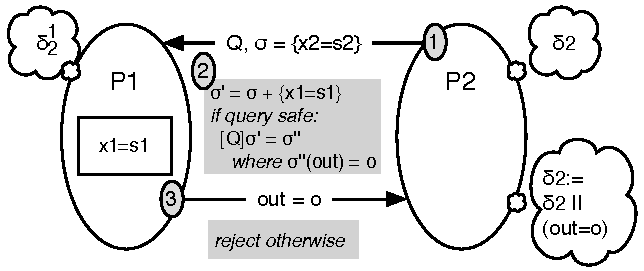
\includegraphics{asymmetric}}
\caption{Asymmetric belief tracking}
\label{fig:asymmetric}
\end{figure}

\begin{figure}[t]
\[
\begin{array}{l}
\polc(q, \delta_i, t_j, x_j) \defeq \\
\\[-2ex]
~_1\quad \underline{\delta_i} := \pevalp{q}\delta_i \\
~_2\quad \kw{forall}\;\emph{possible outputs}\; o\; \\
~_3\quad\quad \hat{\delta_i} := \project{(\revise{\underline{\delta_i}}{(out =  o)})}{\{x_j\}} \\
~_4\quad\quad \kw{if}\; \exists n.\; \hat{\delta_i}(\{x_j = n \}) > t_j\;\kw{then} \\
~_5\quad\quad\quad \kw{return}\; \emph{reject} \\
~_6\quad \kw{return}\; \emph{accept}
\end{array}
\]
% \begin{enumerate}
% \item Let $\underline{\delta_i^j} = \pevalp{q}\delta_i^j$
% \item For all possible outputs $o$
% \begin{enumerate}
% \item Let $\hat{\delta_i^j} = \project{(\revise{\underline{\delta_i^j}}{(out =
%     o)})}{\{x_j\}}$
% \item If there exists an value $v$ such that
%   $\hat{\delta_i^j}(\{x_j = v \}) > t_j$, then $q$ is rejected.
% \end{enumerate}
% \end{enumerate}
\caption{Threshold policy decision, \polc} \label{alg:policy}
\end{figure}

Our prior work~\cite{mardziel11belief} uses Clarkson et al's technique
as a key building block for handling the scenario given in
Figure~\ref{fig:asymmetric}.  Here, in step 1 $P_2$ sends a query $Q$
and a state $\sigma$ to $P_1$.  In step 2, $P_1$ decides whether $Q$
is safe to compute, and if so, executes $\pevalp{Q}{\sigma'} =
\sigma''$, where $\sigma'$ is $\sigma$ with the added mapping of $x_1$
to $P_1$'s secret $s_1$.  In step 3, $P_1$ sends back the result
$o = \sigma''(out)$ if the query was safe, and otherwise rejects the
query.  $P_2$ revises its belief $\delta_2$ based on the outcome.

The main question to answer is how $P_1$ determines whether $Q$ is
safe, i.e., whether it ``reveals too much information.''
%  One natural idea is to use a quantitative measure, e.g.,
% ``reveal no more than $n$ bits of information.''  However, this
% quantitative measure is unsatisfying because it fails to take into
% account what the potential adversaries know, e.g., due to the results
% of prior queries.  \mwh{Say more about this, referring to prior
%   example above; or cut it if we don't care} \pxm{I think the issue
%   here is about relative vs absolute measures of adversary knowledge,
%   we could certainly measure absolute bits in adversary knowledge,
%   say, using relative entropy between belief and actual secret.}
We propose that principal $P_1$ assign to its secret a \emph{knowledge
  threshold} $t_1$, where $0 < t_1 \leq 1$, interpreted to mean that
$P_2$ should never be certain of $P_1$'s secret with probability
greater than $t_1$.  Returning to Example~\ref{ex:q0}, suppose that
$P_1$'s knowledge threshold $t_1 = 1/10$ and $x_1 = 3$. Running $Q_0$
produces $\sfalse$, and $P_2$'s revised belief $\delta_2'$ assigns to
the state $\{ x_1 = 3, out = \sfalse \}$ the probability $1/7$, which
exceeds the threshold.  As such $P_1$ ought to reject
the query.  On the other hand, if the threshold was $1/2$, then the
query could be accepted.

Keeping this intuition in mind, here is how the part notated \emph{is
  the query safe} in Figure~\ref{fig:asymmetric} is implemented.
First, $P_1$ \emph{estimates} $P_2$'s belief $\delta_2$ about $P_1$'s
secret value. We write $\delta^1_2$ to indicate this
estimate.\footnote{How $P_1$ comes by this estimate is beyond the
  scope of this paper, but we point out that for many kinds of data,
  good estimates are easy to come by.  For example, generic
  distributions over personal information like gender, birthday,
  social security number, income, etc. can be gained from census data
  or other public and private repositories (e.g., Facebook
  demographics).} %~\cite{facebook-demographics}).}
  Then $P_1$ calls
\polc$(Q,\delta^1_2,t_1,x_1)$, the pseudocode for which is given in
Figure~\ref{alg:policy}.  Here, $\delta_i$ is bound to $P_1$'s
estimate $\delta^1_2$, while $t_j$ and $x_j$ are bound to $t_i$ and
$x_i$ (that is, the \emph{variable name} $x_i$, not the value it is
bound to), respectively.

On line~1, $P_1$ probabilistically executes $\pevalp{Q}\delta_i$
producing $\underline{\delta_i}$.
%   (In the pseudocode we write
% $\delta_i$, but in fact when $P_1$ executes this function, he provides
% its estimate $\delta_i^1$.)
Then, for each possible output $o$ (line~2), $P_1$ can revise the
belief, $\revise{\underline{\delta_i}}{(out = o)}$, from which we can
project states to involve only secret $x_1$, written $\hat{\delta_i} =
\project{(\underline{\delta_i} | (out = o))}{\{x_1\}}$ (line~3). We
explain shortly why every possible output must be considered, rather
than just the output for $P_1$'s actual secret value.  On line~4, we
check whether for $o$ and corresponding revised belief $\hat{\delta_i}$ there
exists a possible value $n$ such that $(\hat{\delta_i})(\{x_1 = n \}) >
t_1$.  If so, the query $Q$ must be rejected, to avoid leaking
too much information (line~5).  Otherwise, the query is acceptable
(line~6).

If \polc$(Q,\delta^1_2,t_1,x_1)$ returns \emph{accept} then $P_1$ can
execute the query, send back the result, and update its estimate
$\delta_2^1$ to be $\revise{\underline{\delta_2^1}}{(out = o)}$.

\paragraph*{Avoiding leakage due to query rejection.}
Line~2 in Figure~\ref{alg:policy} requires we consider all possible
outputs $o$.  At first glance, doing so seems unnecessarily
conservative.  For Example~\ref{ex:q0}, suppose that $t_1 = 1/5$ and
$\delta^2_1 = \delta_2$; then executing
\polc$(Q_0,\delta^1_2,t_1,x_1)$ would produce \emph{reject}.  But if
the actual secret is $x_1 = 3$, then we have already established that
answering the query (with $\sfalse$) results in $\delta_2$ being
revised to assign $\{ x=3, out=\sfalse \}$ probability $1/7$ which is
below the threshold.  On the other hand, suppose that $x_1$ was $8$
instead of $3$, in which case answering the query with $\strue$ would
cause $P_2$'s revised belief to ascribe probability $1/3$ to $\{ x_1 =
8, out = \strue \}$, which exceeds the threshold $t_1 = 1/5$. But if
$P_1$ rejects the query, and $P_2$ knows threshold $t_1$ it will be
able to infer that the only reason for rejection would be that the answer would
have been $\strue$.  Even if $t_1$ is not known directly, it can be
inferred by enough queries to eventually make this sort of
determination.  $P_1$ avoids this situation by rejecting any query
for which there exists a secret that could be compromised by the
answer, even if that does not happen to be its secret. This approach
results in $ P_1 $ deciding to allow a query or not independetly of
his true secret value. Such policy decisions are \emph{simulatable}
\cite{kenthapadi05simulatable} in that $ P_2 $ could have determined
on their own whether $ P_1 $ will reject the query, hence learning of
$ P_1 $'s decision tells them nothing.

% \subsection{Preventing excessive disclosure}

\section{Enforcing knowledge thresholds for SMC}
\label{sec:SMC-KBSE}

In this section we show how to generalize knowledge-based enforcement
from the single-secret scenario given in Figure~\ref{fig:asymmetric}
to the multi-secret setting of SMC.  In this
setting, there are $N$ principals, $P_1, ..., P_N$ each with a secret
$x_1 = s_1, ..., x_N = s_N$.  Each $P_i$ maintains a belief $\delta_i$
about the possible values of the other participating principals'
secrets.  In addition, each $P_i$ has a knowledge
threshold $t_i$ that bounds the certainty that the other principals
can have about its secret's value.

Next we present an example to
illustrate how belief estimation is adapted to the SMC case, and then
we use this example to illustrate two possible methods we have devised
for enforcing the knowledge threshold, the \emph{belief set} method
(Section~\ref{sec:belief-set}) and
the \emph{SMC belief tracking} method
(Section~\ref{sec:SMC-belief-tracking}).  We prove both methods are
sound and discuss their tradeoffs in Section~\ref{sec:evaluation}.

\subsection{Running example}

Suppose we have three principals, $P_1$, $P_2$, and $P_3$, each with a
net worth $x_1 = 20$, $x_2 = 15$, and $x_3 = 17$, in millions of
dollars, respectively.  Suppose they wish to compute $Q_1$ which
determines whether $P_1$ is the richest:
$$
\begin{array}{lcl}
Q_1 & \defeq  & \sifk\; x_1 \geq x_2 \wedge x_1 \geq
  x_3 \\
&& \quad  \sthenk\;\sassign{out}{\strue} \\
&& \quad \selsek\; \sassign{out}{\sfalse}
\end{array}
$$
Using the idealized view, each of $P_1$, $P_2$, and $P_3$ can be seen
as sending their secrets to $P_T$, which initializes $\sigma$
such that $\sigma(x_1) = 20$, $\sigma(x_2) = 15$, and $\sigma(x_3) =
17$.  Running $Q_1$ using $\sigma$ produces
an output state $\sigma'$ such that $\sigma'(out) = \strue$.

Now suppose that $P_1$ believes that both $P_2$ and $P_3$ have at
least \$10 million, but less than \$100 million, with each case
equally likely.  Thus principal $P_1$'s belief is defined as
$$\begin{array}{l@{}l}
\delta_1 \defeq \lambda \sigma. & \aif \sigma(x_2) < 10\; \aor \sigma(x_2) >
  100\; \aor \\
& \quad \sigma(x_3) < 10\; \aor \sigma(x_3) > 100\; \aor \\
& \quad \sigma(x_1) \not= 20\;\athen 0\; \aelse 1/8281
\end{array}
$$
States which ascribe either $x_2$ or $x_3$ a net worth outside
the expected range, or ascribe $x_1$ to the wrong value, are
considered impossible, and every one of the
remaining 8281 (that is $91 \times 91$) states is given probability
$1/8281$.  The beliefs of $P_2$ and $P_3$ are defined similarly.

% $$\begin{array}{ll}
% \delta_2 \defeq &
% \lambda \sigma\!\in\!\{x_1,x_3\}.\, \aif \sigma(x_1) < 10 \vee \sigma(x_1) >
%   100 \; \athen 0 \\
% & \quad \aelse \aif \sigma(x_3) < 10 \vee \sigma(x_3) > 100\;
% \athen 0 \\
% & \quad \aelse 1/8281 \\
% \delta_3 \defeq &
% \lambda \sigma\!\in\!\{x_1,x_2\}.\, \aif \sigma(x_1) < 10 \vee \sigma(x_1) >
%   100 \; \athen 0 \\
% & \quad \aelse \aif \sigma(x_2) < 10 \vee \sigma(x_2) > 100\;
% \athen 0 \\
% & \quad \aelse 1/8281
% \end{array}
% $$

Belief revision proceeds as before: once $P_T$ performs the
computation and sends the result, each $P_i$ revises its belief.  For
our example query $Q_1$, principal $P_1$ would perform
$\pevalp{Q_1}{\delta_1} = \delta_1''$ and since the output of the
query is $\strue$, then revision produces $\delta_1' =
\dcond{\pevalp{Q_1}{\delta_1}}{\paren{out = \strue}} $.  This revised
belief additionally disregards states that ascribe $x_2$ or $x_3$ to
values greater than $P_1$'s own wealth, which is \$20M:
$$\begin{array}{l@{}l}
\delta_1' \defeq \lambda \sigma. & \aif \sigma(x_2) < 10\; \aor \sigma(x_2) >
  20\; \aor \\
& \quad\sigma(x_3) < 10\; \aor \sigma(x_3) > 20\; \aor \\
& \quad \sigma(x_1) \not= 20\;\athen 0\; \aelse 1/121
\end{array}
$$
The revised beliefs of $P_2$ and $P_3$ will be less specific, since
each will simply know that $P_1$'s wealth is at least their own and no
less than the rest of the parties.

%  Since we assume that $t_i = 1$, $P_1$ can ask
% $P_i$ for its ``secret'' $x_i$ to help initialize this estimate.

% After running $q_1$ and $q_2$, no principal knows any of the others'
% secrets, with the most informed being $P_1$.  But the situation could
% actually have been worse: if both $x_2$ and $x_3$ had been 20 instead,
% then $P_1$'s belief after running $q_1$ would have been just as above,
% but after running $q_2$ the belief would be the point distribution on
% $x_2 = 20$ and $x_3 = 20$; i.e., he would know their secrets exactly!
% Indeed, $P_2$ and $P_3$ would also have the same exact knowledge.
% Since the point of participating in SMC is to avoid revealing the
% secret inputs, this is a poor state of affairs, and one will redress
% in the next section.

% The simple view of SMC we have just given maps directly
% to their approach as follows.

% \paragraph*{Example.}  Returning to our example, suppose $P_1$ has a
% threshold $t_1 = 1/5$ whereas $t_2 = t_3 = 1$ and as such $x_2$ and
% $x_3$ are known to all participants. We suppose that each of the
% beliefs of $P_1$, $P_2$, and $P_3$ are, respectively,
% $$\begin{array}{r@{}l@{}l}
% \delta_1 & \defeq \lambda
% \sigma. & \aif \sigma(x_1) = 20\;\aand \sigma(x_2) = 15 \;\aand
% \sigma(x_3) = 17 \\
% &&  \athen 1\; \aelse 0 \\
% %
% \delta_2 = \delta_3 & \defeq \lambda \sigma. & \aif \sigma(x_1) < 10 \;\aor
% \sigma(x_1) > 100  \\
% && \aor \sigma(x_2) \not= 15\; \aor \sigma(x_3) \not= 17\;
% \athen 0\; \aelse 1/91 \\
% %
% \end{array}
% $$

% To decide whether to participate in $q_1$, suppose principal $P_1$ estimates
% $P_2$'s and $P_3$'s beliefs about the others' secrets exactly, i.e.,
% $\delta_2^1 = \delta_2$ and $\delta_3^1 = \delta_3$. Then $P_1$
% performs computation $\pevalp{q}\delta_2^1 $.  This produces output
% distribution $\underline{\delta_2^1}$, defined as follows:
% $$\begin{array}{l@{}l}
% \underline{\delta_2^1} \defeq \lambda \sigma. &
% \aif \sigma(x_1) < 10 \;\aor \sigma(x_1) > 100 \\
% & \aor \sigma(x_2) \not= 15 \;\aor \sigma(x_3) \not= 17\;  \athen 0 \\
% & \aelse\; \aif x_1 \geq 17 \;\aand out = \strue \; \athen 1/91 \\
% & \aelse\; \aif x_1 < 17 \;\aand out = \sfalse\; \athen 1/91\;
% \aelse 0
% \end{array}
% $$

% Given this output distribution, $P_1$ conditions on the two possible
% outputs, $out = \strue$ and $out = \sfalse$.  Revision in the
% first case produces a distribution that gives each $17 \leq x_1 \leq
% 100$ a $1/84$ chance, so in each case the likelihood of a particular
% value is below the threshold $t_1 = 1/5$.  Revision on the second
% case gives each $10 \leq x_1 < 17$ a $1/7$ chance, which again is
% smaller than $t_1$.  As such, $P_1$ deems the query $q_1$ safe for
% $P_2$.  An identical computation would deem the query safe for $P_3$,
% since $\delta_3^1 = \delta_2^1$, and so $P_1$ would agree to
% compute $q_1$ and share the result (which is $\strue$).  Afterward
% $P_1$ would revise $\delta_2^1$ to be $\revise{\underline{\delta_2^1}}{(out =
%   \strue)}$, which is
% $$\begin{array}{l@{}l}
% {\delta^1_2}' \defeq \lambda \sigma. &
% \aif \sigma(x_1) \leq 17 \;\aor \sigma(x_1) > 100 \\
% & \aor \sigma(x_2) \not= 15 \;\aor \sigma(x_3) \not= 17\;  \athen 0\;
% \aelse 1/84
% \end{array}
% $$
% and do likewise for $\delta_3^1$.

% \paragraph*{Avoiding leakage due to query rejection.}
% Now suppose instead that $t_1 = 1/20$. In this scenario, $P_1$ would
% refuse to participate because in the case that the output were
% $\sfalse$, he would estimate that $P_2$ and $P_3$ could guess his
% secret with probability $1/7 > 1/20$.  But in fact, the output will be
% $\strue$, not $\sfalse$, so were the query is actually performed the
% probability will be $1/84$; we would seem to have rejected query
% unnecessarily.

% The key question is: why must $P_1$ consider \emph{every} possible
% output and not just the output that would result from his actual
% secret?  The reason is because rejection of a query would then reveal
% information.  To see why, suppose that $x_1$ was $12$ instead of $20$,
% in which case answering the query with $\sfalse$ gives $P_2$ and $P_3$ too much
% information.  If $P_1$ rejects the query, and the threshold $t_1$ is
% known, $P_2$ and $P_3$ will know that the only reason for rejection
% would be that the answer would have been $\sfalse$.  Even if $t_1$ is
% not known directly, it can be inferred by enough queries to eventually
% make this sort of determination.  $P_1$ avoids this situation by
% rejecting any query such that there exists a secret that could be
% compromised by the answer, even if that does not happen to be his
% secret. This approach results in $ P_1 $ deciding to allow a
% query or not independetly of his true secret value. Such policy
% decisions are \emph{simulatable} \cite{kenthapadi05simulatable} in
% that $ P_2 $ (or $ P_3 $) could have determined on their own whether $
% P_1 $ will reject the query, hence learning of $ P_1 $'s decision
% tells them nothing.

% For example, suppose $f(x,y) \defeq x > y$ and $x_2 = 5$.  Then
% $f(\delta^2_1,5) | \emph{true}$ is a distribution $\delta_\emph{true}$
% such that $\delta_\emph{true}(i) = 1/360$ for $i > 5$ and
% $\delta_\emph{true}(i) = 0$ for $i \leq 5$.  On the other hand,
% $f(\delta^2_1,5) | \emph{false}$ is a distribution
% $\delta_\emph{false}$ such that $\delta_\emph{false}(i) = 0$ for $i >
% 5$ and $\delta_\emph{false}(i) = 1/5$ for $i \leq 5$.  Suppose $t_1 =
% 0.1$.  Then $p_1$ will reject $f$ because there exists a possible
% valuation of the secret $x_1$ (i.e., when $1 \leq x_1 \leq 5$) such
% that the attacker learns too much.  For $t_1 = 0.3$, then $f$ would be
% accepted since neither output induces a belief in a value that exceeds
% the threshold.  The actual result $f(x_1,5)$ is returned to $p_2$, and
% the belief $\delta^2_1$ is updated to be either $\delta_\emph{true}$
% or $\delta_\emph{false}$ depending on the actual result.  This updated
% belief is used for subsequent requests.


\subsection{Knowledge-based security with belief sets}
\label{sec:belief-set}

% Suppose each $P_i$'s knowledge threshold about his personal wealth is
% $1/10$.  Then after $q_1$, this threshold is satisfied: the most
% knowledgable principal is $P_1$ and he believes that values from $10
% .. 20$ are equally likely for each of $x_2$ and $x_3$, i.e., each with
% a $1/11$ probability.


% $P_1$ follows roughly the same procedure as above, but instead of
% maintaining a single distribution $\delta_i^1$ for each remote party
% $P_i$, it maintains a \emph{set} of distributions $\Delta_i^1$, where
% each distribution in the set applies to a particular valuation of
% $x_i$.

Now we wish to generalize threshold enforcement, as described
in Section~\ref{sec:kbse}, to SMC\@.  In the simpler setting $P_1$ maintained an
estimate $\delta_2^1$ of $P_2$'s belief $\delta_2$.  In the SMC setting
we might imagine that each $P_j$ maintains a belief estimate
$\delta_i^j$ and then performs \polc$(q,\delta_i^j,t_j,x_j)$ for all
$i \not= j$.  If each of these checks succeeds, then $P_j$ is willing
to participate.

The snag is that $P_j$ cannot accurately initialize $\delta^j_i$ for
all $i \not= j$ because it cannot directly represent what $P_i$ knows
about $x_i$---that is, its exact value.  So
the question is: how can $P_j$ estimate the potential gain in $P_i$'s
knowledge about $x_j$ after running query without knowing $x_i$?

One approach to solving this problem, which we call the \emph{belief
  set} method, is the following.
$P_j$ follows roughly the same procedure as above, but instead of
maintaining a single distribution $\delta_i^j$ for each remote party
$P_i$, it maintains a \emph{set} of distributions where each
distribution in the set applies to a particular valuation of $x_i$.
As a first cut, suppose that $P_j$ initializes this set to be as
follows:
$$
\Delta_i^j \defeq \{\revise{\delta^j_i}{(x_i = v)} \given v = \sigma(x_i),
\sigma \in \nzset{\project{\delta_j}{\{x_i\}}}\}
$$
Thus $\Delta_i^j$ is a set of
possible distributions, one per possible valuation of $x_i$ that $P_j$ thinks
is possible according to its belief $\delta_j$.

\pxm{This ``flawed'' definition has some problems outside of the one
mentioned below. There is no $ \delta^j_i $ as was mentioned in the
paragraphps preceeding. We had a cross product based construction here
before but that required us to explain cross product and some other
things. Can we make due by just introducing the ``non-flawed''
approach directly?}
\mwh{Noticed that, did you? :)  I was going to try to sneak it past
  the reader, but you're right.  I'd rather leave this here to give a
  sense of where we're going.  We can talk more about it, e.g., for
  the final submission tomorrow.}

However, this method for initializing the set is not quite expressive
enough, since it may fail to take into account correlations among
beliefs of multiple principals.  For example, if it were known (by all
principals) that only one of the principals in the running example can
have secret value equal to 15, then $ P_2 $ would know initially,
based on this own secret $ x_2 = 15 $, that $ P_1 $'s value $ x_1 $
cannot be $ 15 $. However, $ P_1 $ cannot arrive at this conclusion
without knowing $ x_2 $, which is, of course, outside of its knowledge
initially.

Therefore, we define the initial belief set using a distribution $
\delta $ over \emph{all} principals' secret data which sufficiently
captures any correlations in those secrets. Such a distribution can
then be used, given some valuations of secret variables, to derive
what a principal's initial belief would be.
$$
\Delta_i \defeq \{\revise{\delta}{(x_i = v)} \given v = \sigma(x_i), \sigma \in \nzset{\project{\delta}{\{x_i\}}} \}
$$
Since we are starting from a globally held belief $\delta$, there is
no need to distinguish $\Delta_i^j$ from $\Delta_i^k$---they
are the same $\Delta_i$.

\begin{figure}
\scalebox{.8}{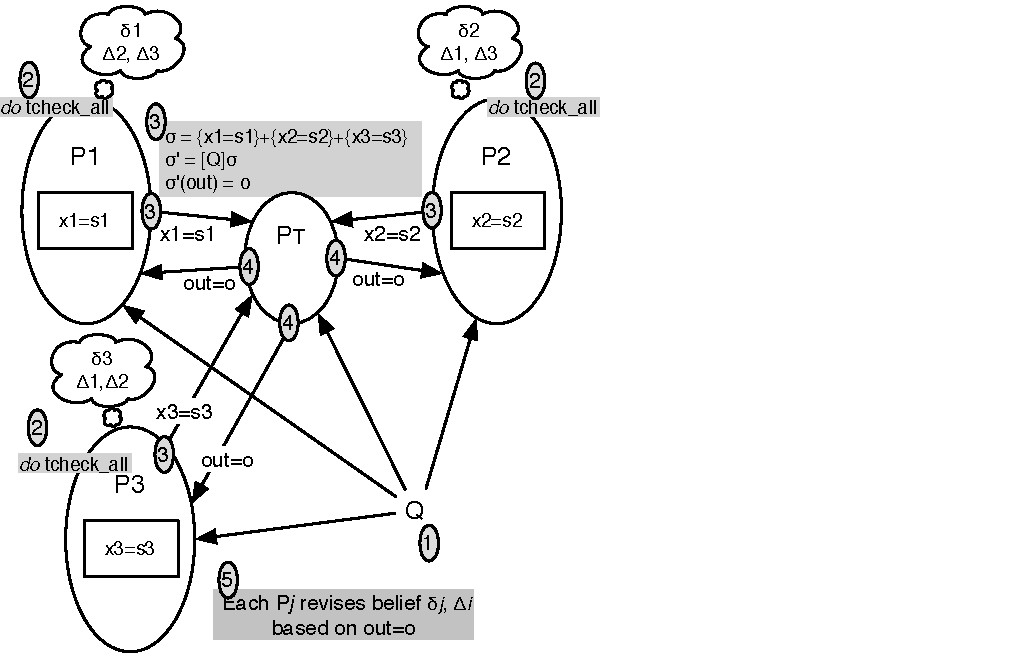
\includegraphics{symmetric}}
\caption{Threshold enforcement for SMC using belief sets}
\label{fig:smc-sets}
\end{figure}

\begin{figure}[t]
\[
\begin{array}{l}
\polcall(q, j) \defeq \\
\\[-2ex]
~_1\quad \kw{forall}\;i \in 1..n\;\kw{with}\; i \not= j \\
~_2\quad\quad \polc(q,\Delta_i,t_j,x_j) \\
~_3\quad\kw{if}\; \emph{all threshold checks succeed}\; \kw{then} \\
~_4\quad\quad \emph{agree to participate} \\
~_5\quad\kw{else} \\
~_6\quad\quad \emph{refuse to participate} \\
\end{array}
\]
\caption{\polcall{} check for belief set enforcement}
\label{alg:belief-set-check}
\end{figure}

Now each $P_j$ follows the procedure depicted in
Figure~\ref{fig:smc-sets} for the idealized view (with a trusted
principal $P_T$).  First, the principals agree on the query $Q$.
Second, each principal $P_j$ performs the threshold check
\polcall$(Q,j)$, whose code is given in Figure~\ref{alg:belief-set-check}.
Notice that calls to \polc(...) on line~2 are with the set $\Delta_i$, rather
than a single distribution $\delta_i^j$.  The definitions of the
operations in the pseudocode in Figure~\ref{alg:policy}, when applied
to sets $\Delta$ rather single elements $\delta$, are defined in
Figure~\ref{fig:sem-sets}.  In
all but the last case, these operations are just straightforward
liftings of the operations on single distributions.  For
$\Delta(\sigma)$, we return the highest probability for $\sigma$ of
those ascribed to it by distributions in $\Delta$, to assure that our
decision to participate or not is safe.  Also note that we will always
be dealing with non-empty $ \Delta $, hence the maximum probability is
sufficiently defined. On the other hand, the normalization procedure
for distributions $ \delta $ is only well defined whenever $
\pmass{\delta} > 0 $. Because of this, we make sure the normalization
for distribution sets only normalizes the normalizable distributions,
and discards the rest. The way in which some member distributions of $
\Delta $ could become non-normalizable, that is, having mass of $ 0 $,
is by way of the conditioning operation, where the condition is
inconsistent with all possible states in the distribution.

\begin{figure}
\centering
Semantics
\begin{displaymath}
\begin{array}{l}
\pevalp{S}{\Delta} = \{ \pevalp{S}{\delta} \given \delta \in \Delta \} \\
\end{array}
\end{displaymath}
Operations
\begin{displaymath}
\begin{array}{l@{\;\defeq\;}l}
\project{\Delta}{V} & \{ (\project{\delta}{V}) \given \delta \in \Delta \} \\
\normal{\Delta} & \{
\normal{\delta} \given \delta \in \Delta \; , \; \pmass{\delta} >
0\} \\
\revise{\Delta}{\bexp} & \normal{\{
(\dcond{\delta}{B}) \given \delta \in \Delta \} } \\
\Delta(\sigma) & \max_{ \delta \in \Delta} \delta(\sigma) \\
% \Delta_1 \times \Delta_2 & \{ \delta \mid \delta_1 \in \Delta_1
% \wedge \delta_2 \in \Delta_2 \wedge \delta = \delta_1 \times \delta_2
% \} \\
\end{array}
\end{displaymath}
\caption{Probabilistic semantics using sets of distributions}
\label{fig:sem-sets}
\end{figure}

% \begin{algorithm}[h!]
% \begin{enumerate}
% \item Let $\underline{\Delta_i} = \pevalp{q}\Delta_i$
% \item For all possible outputs $o$
% \begin{enumerate}
% \item Let $\hat{\Delta_i} = \project{(\revise{\underline{\Delta_i}}{(out =
%     o)})}{\{x_1\}}$
% \item If there exists an value $v$ such that
%   $\hat{\Delta_i}(\{x_1 = v \}) > t_1$, then $q$ is rejected.
% \end{enumerate}
% \end{enumerate}
% \caption{Belief set threshold policy decision} \label{alg:sets_policy}
% \end{algorithm}

In the third step, if the query is acceptable for all $P_j$, each sends its
secret $x_j = s_j$ to $P_T$, which executes $Q$
using the secret state $\sigma$ constructed from each secret.  Fourth,
the result $o$ is sent back to each principal.  Finally, as usual,
$P_1$ revises each of its estimates $\Delta_i$ and its own belief
$\delta_j$.  Note that all principals make the same update for
$\Delta_i$, hence
there really is only one $ \Delta_i $, known by all, estimating $ P_i
$'s knowledge.
%  The only difference in the policy is the variables
% projected onto when checking the threshold, that is, $ P_1 $ projects
% onto $ \{x_1\} $, whereas $ P_2 $ would project onto $ \{x_2\} $.

While we have depicted this procedure in the idealized view of SMC, it
is easy to see that we can simply implement steps 3 and 4 as a normal
SMC and the remainder of the procedure is unchanged.

\subsection{Soundness of belief sets}

Now we can show that the belief set procedure is
\emph{sound}, in that for all $P_i$, participating or not
participating in a query will never increase another $P_j$'s certainty
about $P_i$'s secret above its threshold $t_i$.

\begin{remark}
\label{rem:sound-sets}
Suppose principals $P_1, ..., P_N$ wish to execute a query $Q$.  The
secret state $\sigma_s = \{ x_1 = s_1, ..., x_N = s_N \}$ contains all
their secrets.  Assume that for each $P_i$:
\begin{enumerate}
\item $ P_i $ has a belief $ \delta_i $.
\item $ P_i $'s belief $ \delta_i $ is consistent with $ \sigma_s $, that is,
$\delta_i(\sigma_s) > 0 $.
\item $ P_i $'s belief $ \delta_i $ is within the public estimate of
his knowledge, that is, $\delta_i \in \Delta_i$.
% \item \pxm{delete, not needed: and $\delta_i(\sigma) = 0$ for all $\sigma$
% with $\sigma(x_i) \not= v_i$}
\end{enumerate}
Suppose $\pevalp{Q}{\sigma_s} = \sigma_s'$ such that $\sigma_s'(out) =
o$. That is, the actual output of the query $Q$ is
$o$. Then, the belief of each agent, after learning the output, is
$ \revise{\delta_i}{(out = o)} $, and is a member of the estimated set
$ \revise{\Delta_i}{(out = o)} $.
\end{remark}

\begin{proof}
\tref{thm:clarkson} tells us that $\delta_i' =
\revise{\pevalp{Q}{\delta_i}}{(out = o)}$ are the new beliefs of the
principals, having learned that $ out = o $. By assumption we had
$ \delta_i \in \Delta_i $, and since $ \delta_i $ was consistent with
$ \sigma_s $, it must be that $ \delta'_i $ is consistent (having
non-zero mass), and therefore $ \delta'_i \in \Delta'_i
= \revise{\Delta_i}{(out = o)}$.
\end{proof}

This remark is merely a lifting of \tref{thm:clarkson} to
sets of beliefs. The more interesting point arises when the principals
are also interested in enforcing a knowledge threshold.

\begin{lemma}
\label{lem:sound-sets}
Suppose the same premise as \rref{rem:sound-sets}. Also suppose that
policy thresholds $t_i$ are public, and $\pevalp{Q}{\sigma_s} = \sigma_s'$
such that $\sigma_s'(out) = o$. That is, the actual output of the
query $Q$ is $o$, and each $P_i$ learns either
\begin{itemize}
\item the output $ o $ of the query, or
\item which principals $P_j$ rejected the query.
\end{itemize}
Then, the belief of each agent, in the first case is
$ \revise{\delta_i}{(out = o)} $, and is within the estimate
$ \revise{\Delta_i}{(out = o)} $, or in the second case, remains at
$ \delta_i $.
\end{lemma}
\begin{proof} The lemma effectively states that the policy decisions
have no effect on the beliefs; if a query is
rejected, learning which principals rejected it reveals
nothing. Similarly, if the query is not rejected, the additional
information each principal gets (that no one rejected the query), also
does not change the belief.

The lemma holds due to the simple fact that the policy decisions do
not depend on private information (see \fref{alg:belief-set-check}),
every single principal could determine, on their own, whether another
principal would reject a query. Thus the policy decisions, as a whole,
are a simulatable procedure. The rest follows
from \rref{rem:sound-sets}.
\end{proof}

Some subtleties are worth mentioning.  First, a premise of the lemma is that
$ \Delta_i $ are known by all principals. This fact
needs to remain as the query is answered so the same premise will
hold for the next query. Fortunately this is the case, as the revised belief
sets in the case of policy success, $ \revise{\Delta_i}{out = o} $ are
also known by all participants, as $ o $ is known, and so are the
initial $ \Delta_i $.

A second subtlety is that the queries themselves must be chosen
independent of anyone's secret. In some situations, where the
principals are actively attempting to maximize their knowledge, and
are allowed to propose queries to accomplish this, the query choice
can be revealing. This problem is beyond the scope of this work, and
we will merely assume the query choice is independent of secrets.

% \pxm{the rest can probably be moved or deleted}
% First, if $P_i$ chooses to reject the query, then it does so without
% considering the actual secrets of any other participants.  Therefore
% rejection does not reveal any information.  \mwh{Perhaps the previous
%   statement is the hole in this argument?}

% Second, if $P_i$ chooses to go ahead, we know that he does so based on
% all possible outputs $o$, so it will consider ${\Delta_j^i}'$ (for all
% $j \not= i$) since this revision is based on the true output (one of
% the possibilities).  Moreover, the threshold check will fail if there
% exists any $\delta \in {\Delta_j^i}'$ such that
% $(\project{\delta}{\{x_i\}})(x_i) > t_i$, but since we know that
% $\delta_j' \in {\Delta_j^i}'$ then it must be that
% $(\project{\delta_j'}{\{x_i\}})(x_i) \leq t_i$, and thus the threshold
% check is satisfied.

% Moreover, it is clear that whether or not we go ahead with the query,
% Lemma~\ref{lem:sound-sets} reestablishes the two conditions needed to
% apply it to any subsequent query.  In particular, if we reject the
% query, then the conditions trivially remain satisfied.  If we accept
% the query, then condition (1) follows from the semantics of belief
% revision: if the true state was considered a possibility before the
% query, then a revision based on the output of the query operating over
% the true state must leave the true state a possibility \mwh{presumably
%   this is some lemma from Clarkson we can prove}. Condition (2) is the
% result of the lemma, so it is trivially satisfied.

\begin{figure}[t]
\scalebox{.8}{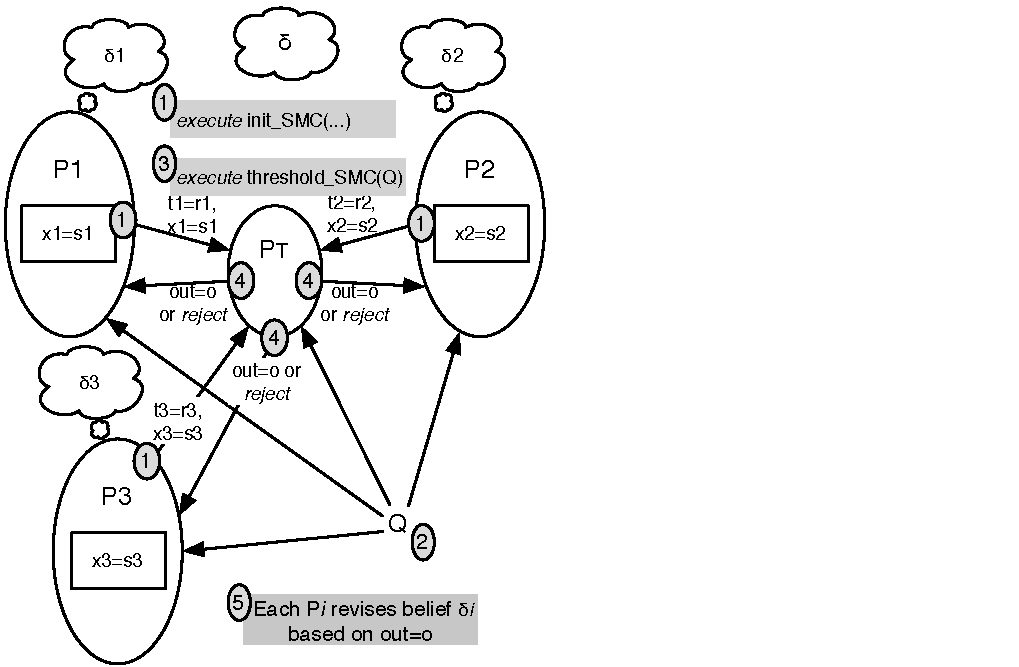
\includegraphics{symmetric-SMC}}
\caption{SMC belief tracking scenario (ideal view)}
\label{fig:belief-smc}
\end{figure}

\begin{figure}[t]
\[
\begin{array}{l}
\mathsf{init\_SMC}(s_1...s_N,r_1...r_N,\delta) \defeq \\
\\[-2ex]
~_1\quad\, \sigma_s := \{ x_1 = s_1, ..., x_N = s_N \} \\
~_2\quad\, \delta_1 := \revise{\delta}{(x_1 = s_1)};\; t_1 := r_1 \\
~~~~~~~~~~... \\
~_{n\!+\!1}\; \delta_N := \revise{\delta}{(x_N = s_N)};\; t_N := r_N \\
\\
\mathsf{threshold\_SMC}(Q) \defeq \\
%\\[-2ex]
~_1\quad o := (\pevalp{Q}{\sigma_s})(out) \\
~_2\quad \kw{forall}\;j \in 1..n \\
~_3\quad\quad \kw{forall}\;i \in 1..n\; \kw{with}\; i \not= j \\
~_4\quad\quad\quad \polc(Q,\delta_j,t_i,x_i) \\
~_5\quad\quad \kw{if}\; \emph{all threshold checks succeed}\; \kw{then} \\
~_6\quad\quad\quad \delta_j := \revise{\pevalp{Q}{\delta_j}}{(out = o)} \\
~_7\quad\quad\quad \kw{return}\;o\;\kw{to}\;P_j \\
~_8\quad\quad \kw{else} \\
~_9\quad\quad\quad \kw{return}\;\emph{reject}\;\kw{to}\;P_j
\end{array}\]
\caption{SMC belief tracking (ideal view)} \label{fig:threshold-mc-alg}
\end{figure}

\subsection{SMC belief tracking: ideal world}
\label{sec:SMC-belief-tracking}
Now we present an alternative to the belief set method, in which the
decision to participate or not, involving checking thresholds after
belief revision, takes place \emph{within the SMC itself}.  As such,
we call this method \emph{SMC belief tracking}.
Once again we present the algorithm using the ideal world with a
trusted third party $P_T$.  The steps are shown in
Figure~\ref{fig:belief-smc}.  The first step is that each $P_i$
presents its secret $x_i = s_i$ to $P_T$, along with the collective
belief $\delta$.  Principal $P_T$ then initializes the computation state by
calling $\mathsf{init\_SMC}(s_1...s_N,\delta)$, given in
Figure~\ref{fig:threshold-mc-alg}.  On line~1, this code initializes
the secret state $\sigma_s$ that contains all of the secrets.  On
lines~$2..(n\!+\!1)$, it initializes each principal $P_i$'s belief
as in the belief set case, by specializing $\delta$ with the
knowledge unique to $P_i$.  It also initializes each threshold $t_i$ to
$r_i$.

In step 2 (of the diagram), the query $Q$ is made available to $P_T$,
which then runs (in step 3) $\mathsf{threshold\_SMC}(Q)$, also shown
in Figure~\ref{fig:threshold-mc-alg}.  On line~1 we compute the actual
output $o$ for the query, based on the secret state.  On line~2 we
loop over each principal $P_j$.  The remainder of the code aims to
decide whether answering the query and sending the result to $P_j$
would reveal too much information; if not, we send $P_j$ the answer
$o$ (line~7) and otherwise we reject.

Returning to the body of the loop, the
next step is to make sure that for every $P_i$ (line~3) its threshold
check (Figure~\ref{alg:policy}) will not reject $P_j$.  That is, given
the query $q$ and the estimated knowledge of $P_j$, we make sure that
the answer to the query will not reveal too much about $P_i$'s secret
$x_i$ (where by ``too much'' we mean $P_j$'s certainty about $P_i$'s
possible secret exceeds threshold $t_i$).  Assuming all $P_i$
threshold checks succeed (line~5), we then revise the $P_j$'s belief
according to the output $o$ (line~6), which we then send to $P_j$
(step 4 in the diagram).  No
revision is done on $P_j$'s belief if the query is rejected for
$P_j$. Finally, each principal revises its own belief $\delta_j$ based
on the output.

We can repeat steps 2--5 for each subsequent query $Q'$, and $P_T$
will use any beliefs $\delta_j$ revised from the run of $Q$.  By
performing \textsf{threshold\_SMC} as part of an SMC, no participant
$P_i$ is ever shown the opposite's secret, and yet an accurate
determination is made for each about whether to participate.

Importantly, the fact that $P_j$ receives a
proper answer or \emph{reject} is not (directly) observed by any other
$P_j$; such an observation could reveal information to $P_j$ about
$x_i$. For example, suppose $Q_2 \defeq x_1 \leq x_2$ and both secrets
are (believed to be) between 0 and 9.  If $x_2 = 0$ then
$\pevalp{Q_2}{\sigma_s}$ will return $\strue$ only when $x_1$ is also
$0$.  Supposing $t_1 = 3/5$, then $P_2$ should receive \emph{reject}
since there exists a valuation of $x_1$ (that is, 0) such that $P_2$
could guess $x_1$ with probability greater than $3/5$.  Similar
reasoning would argue for reject if $x_2 = 9$, but acceptance in all
other cases.  As such, if $P_1$ observes that $P_2$ receives
\emph{reject}, it knows that $x_2$ must be either $0$ or $9$,
independent of $t_2$; as such, if $t_2 < 1/2$ we have violated the
threshold by revealing the result of the query.

This asymmetry means that \textsf{threshold\_SMC} may return a result
for one participant but not the other, e.g., $P_1$ might receive
\emph{reject} because $t_2$ is too low while $P_2$ receives the actual
answer because $t_1$ is sufficiently high.  Nonetheless each $P_i$'s
threshold will be respected.

\subsection{SMC belief tracking: real world}

Lacking a trusted third party in the real world, the participants
can use secure multi-party computation and some standard
cryptographic techniques to implement $ P_T $'s functionality amongst
themselves. There are two aspects of $ P_T $ that they need to handle:
the computation $ P_T $ performs, and the hidden state $ P_T $
possesses in between queries.

The first aspect is exactly what SMC is designed to do. For the second
aspect, we need a way for the participants to maintain $ P_T $'s state
amongst themselves while preserving its secrecy.  (Since we are using
the semi-honest adversary model, we do not concern ourselves with
integrity; in the malicious setting, standard techniques could be used
to enforce integrity.) This
state, initially constructed by $ \mathsf{init\_SMC} $
(\fref{fig:threshold-mc-alg}) consists of (1) the parties' secrets,
encoded as a state $ \sigma_s $; (2) policy thresholds $ t_i $; and
(3) the current beliefs $ \delta_i $.  We will refer to this state as
$ \Sigma_T $.\footnote{Technically, secrets $s_i$ and thresholds $t_i$
  could be provided to each invocation of \textsf{threshold\_SMC}; we
  consider them part of the state to emphasize that they are set in
  place initially, and assumed to not change.}
  We assume $\Sigma_T$ can be encoded by a binary string
  of length (exactly)~$\ell$, for some known~$\ell$.

The initialization procedure formulated in the idealized world does
not output anything to the participants. In the real world, however,
the secure computation of $ \mathsf{init\_{SMC}} $ returns \emph{secret shares}
of $\Sigma_T$ to the parties. That is, the secure computation implements
the following (randomized) function after computing~$\Sigma_T$:
choose random $c_1, \ldots, c_{N-1} \in \{0,1\}^\ell$
and set $c_N = \Sigma_T \oplus \left( \bigoplus_{i=1}^{N-1} c_i \right)$. Then each party $P_i$
is given~$c_i$.

The query-evaluation procedure $ \mathsf{threshold\_{SMC}} $ receives
$ (c_1, ..., c_N) $ along with the query $ Q $. The procedure begins by reconstructing
$\Sigma_T = \bigoplus_{i=1}^N c_i$,
and then
proceeds as usual.  Upon completion, $ \mathsf{threshold\_{SMC}} $
computes (new) shares $c'_1, \ldots, c'_N$ of $\Sigma'_T$ (as before), and gives $c'_i$ to~$P_i$
along with the actual output.
(At this point, each $P_i$ can erase the old share~$c_i$.)

% Now, to properly implement the idealized world $ P_T $ in the real
% world, the participants cannot learn anything new from their shares of
% the encoded hidden state. If we further assume the potential of
% dishonest participants, we will also need $ C $ to provide some means
% of integrity assurance, preventing participants from changing the
% hidden state in between $ \mathsf{threshold\_{SMC}} $ invocations.

Note that each time the sharing is done, nothing additional about $\Sigma_T$ is revealed from
any individual fragment (``share'')~$c_i$. (Indeed, each $c_i$ is simply a uniform binary string of length~$\ell$.)
In particular, just as in the ideal world, $P_i$
does not learn whether its policy rejected another participant~$P_j$.
%The encoding $ C $ must ensure that $ P_i $ cannot learn this
%information from his encoding component. This can be accomplished
%either by making $ C $ non-deterministic or by encoding $ \delta_j $
%in $ c_j $, $ P_j $'s component of the shared hidden state (as $ P_j $
%can and does learn whether he was rejected).\footnote{In fact we could
%even let $ P_j $ keep $ \delta_j $ in the clear as they are assumed
%to believe it.}
% \mwh{About keeping it in the clear: does this mean
% that no information is leaked into the belief?  At one point, I
% thought we believed it was.  This fact is indicated in section 5, so
% if it's not true, we should drop the claim.} \pxm{The point made
% before was about, say, $ P_i $ being prevented from seeing $ \delta_j
% $ for $ i \neq j $. $ P_j $, however, can see it, as he is assumed to
% know/believe it.}



% \paragraph{Integrity} Semi-honest participants $P_i$ may be willing
% to tamper with the $c_i$ they provide as a real world input.  To
% address this concern, we require that if $ C(\Sigma_T) = (c_1, ...,
% c_N) $ and $ 1 \leq \setsize{\set{c'_i \given c_i \neq c'_i}} < N $
% then $ C^{-1}(c'_1, ..., c'_N)
% \in \set{\bot, \Sigma_T} $. Here $ \bot $ signifies integrity failure, which is detected if at
% least one, but not all, agent dishonestly reports his encoding
% component. \mwh{This seems wacky: you are not showing any additional
% parameters to $C$, so it seems like it should allow different $c_i$ to
% produce a different $\Sigma_T$.} We could also relax, depending on the
% situation, this condition, detecting integrity failure only when more
% than one participant is dishonest. \pxm{Prof Katz: does this make
% sense? is sufficient? too strong? Existing crypto means to show this
% is implementable?}

% Consequently, we will make use of the mentioned guarantees in our
% soundness analysis. Specifically we have the following remark about
% the connection between the ideal and the real worlds.

\begin{remark} \label{remark:ideal-real} Honest (but curious) participants can derive
exactly the same knowledge about each other's secrets from
the real-world SMC implementation of $ P_T $ that
they do from interacting with $ P_T $ in the idealized world.
%
Specifically, $ P_T $ reveals only the following to each agent $ P_i $ in
the ideal world:
\begin{itemize}
\item{} Output of a query, if policy checks on $ \delta_i $ succeed, or
\item{} rejection, if a policy fails.
\end{itemize}
\end{remark}


%\mwh{Text below is old.  say what happens to the ``shared state'' kept
%  by $P_T$.}
%
%We must make one further adjustment to $Q$.  Instead of returning the
%belief model $\underline{\delta^2_1} | \var{x}$ to $P_1$, $Q$ must
%return the revised belief \emph{encrypted}, and must accept (and
%decrypt) this belief in future computations.  The reason is that the
%revised belief returned $P_1$ could reveal something about $x_2$.  For
%example consider the same $f$ as above with the secrets again being
%between 0 and 9.  Suppose that $P_1$'s initial model of $P_2$'s belief
%$\delta^2_1$ is the uniform distribution between 0 and 9.  Assuming
%the computation is accepted, $Q$ returns, on line 6, the revised
%belief to $P_1$. Suppose $P_1$ could look at the belief and see that
%it is, say, uniform between 4 to 9.  This revised belief would only
%happen if $x_2$ is 4 and hence $P_1$ would know $x_2$ exactly.

% Longer e-mail; may have something useful in it:

% Let's say we have two principals X and Y whose secrets are integers x
% and y and the query Q(x,y) is x > y.  Each principal models the
% other's belief about his secret as a uniform distribution for values
% between 1 and 100, and X has a threshold of 0.1, while Y has a
% threshold of 0.05.  Finally, suppose the actual secrets are x = 50 and
% y = 1.

% In the SMC scenario that you've proposed, as I understand it, there
% will be two distributed belief calculations; the whole thing will be
% rejected if either is rejected.

% First will be X's and the query will be specialized to Y's actual
% value, i.e., Qy(x) = x > 1.  This calculation will reject Q because
% returning false is a possible answer according to Y's belief of x, and
% doing so would reveal x to be 0 or 1, which violates x's threshold of
% 0.1 (i.e., X will only allow Y to know x as one of 10 possibilities,
% but this would narrow it to 2).

% Next will be Y's belief calculation.  This will be specialized to X's
% actual value, i.e., Qx(y) = 50 > y.  In this case, Y will accept the
% query because whether the query returns true or false, the remaining
% possible values of y according to X's belief are above the threshold
% of 0.05 (i.e., Y will only allow X to know y as one of 20
% possibilities, but X, as a result of the query only knows it within
% roughly 50 possibilities).

% Here's the problem: because our attack model assumes that beliefs and
% thresholds are public, X knows that Y's belief calculation will
% succeed.  This is because he knows everything about the calculation:
% his value x, Y's model of his belief about y, Y's threshold, and the
% query Q.  Therefore, if the query is rejected, he knows it is because
% of his belief calculation.  Moreover, because he knows his threshold,
% he can deduce exactly those values of y that would have caused the
% query to be rejected, in particular, 0 <= y < 10.  So, rejection has
% narrowed the number of possibilities for y to be 10, and this violates
% y's threshold.

% You can't easily fix this problem by assuming beliefs and thresholds
% aren't known to all participants because the decision to reject (as
% given above, and defined in our CSF paper) depends on these, and so it
% accepting or rejecting a query reveals information about them.  You'd
% have to come up with a new way of rejecting queries that did not
% reveal information about beliefs, which seems impossible to me, or
% you'd have to reason about how much information about beliefs etc. is
% being communicated and take that into account, but even if you did
% that, you could ultimately wind up in the situation I've given above.

%We can amend $Q$ to generate a random integer $r_1$ and return $r_1$
%to $P_2$ and $(\underline{\delta^2_1} | \var{x}) \oplus r_1$ to $P_1$
%(where $\oplus$ denotes the exclusive-or operation).  We do likewise
%for the $P_2$'s part.  When the two parties next participate in an SMC
%they will provide these two values as inputs to $Q$ so it can decrypt
%the belief.  Note that $Q$ must generate a new random $r_i$ with each
%computation or else $P_i$ could observe that its belief did not
%change, revealing a likely rejection (depending on $f$).
%
%One problem with the SMC approach is that $P_1$ could set its
%threshold or modeled belief so that \emph{reject} is essentially
%always returned to $P_2$, while a more reasonable valuation of these
%inputs by $P_2$ would allow $P_1$ receive the actual answer.  Because
%$P_2$ would not know that $P_1$ is receiving an answer or not, it
%would not realize that it is being gamed.  \mwh{Is this prior
%  statement correct?}

\subsection{Soundness of SMC belief tracking}
Suppose that no dishonest parties are detected during the runs of SMC
belief tracking.  Then, by \rref{remark:ideal-real},
we can justify soundness in the real world by considering the approach in
the idealized world.

\begin{lemma}
\label{lem:sound-smc}
Suppose principals $P_1, ..., P_N$ wish to execute a query $Q$.  The
secret state $\sigma_s = \{ x_1 = s_1, ..., x_N = s_N \}$ contains all
their secrets. Each has a public threshold $ t_i $ for their policy
check.
Assume the following for each $P_i$:
\begin{enumerate}
\item $ P_i $ has a belief $ \delta_i $ about the secret variables.
\item $ P_i $'s belief $ \delta_i $ is consistent with $ \sigma_s $, that is,
$\delta_i(\sigma_s) > 0 $.
\end{enumerate}
Suppose $\pevalp{Q}{\sigma_s} = \sigma_s'$ such that $\sigma_s'(out) =
o$. That is, the actual output of the query $Q$ is
$o$. Then, for each agent $ P_i $:
\begin{itemize}
\item{} If $P_i$ receives output $ o $ from $ P_T $, its revised
  belief is $ \revise{\delta_i}{(out = o)} $.
\item{} If $P_i$ is rejected, its belief does not change.
\end{itemize}
Specifically, in either case, the procedure
$ \mathsf{threshold\_{SMC}} $ maintains the correct beliefs.
\end{lemma}

\begin{proof}
The proof of this lemma reasons similarly
Lemma~\ref{lem:sound-sets}: rejection  reveals nothing new, and
acceptance tracks beliefs precisely.   We can see from
line 4 of \fref{fig:threshold-mc-alg},
that the procedure used to determine whether $ P_j $ will receive
an answer or  rejection depends on four things:
\begin{itemize}
\item{} The query $ Q $, which is assumed to be public, and chosen
independently of secrets.
\item{} $P_j$'s belief, $ \delta_j $, about the secrets. This is
naturally known by $ P_j $. \mwh{Is it?  I thought it could contain
  information, e.g., the fact that someone else was
  rejected.} \pxm{Someone else being rejected would not be reflected
  in $ \delta_j $, only $ P_j $'s rejection is reflected in it.}
\item{} Thresholds $ t_i $ for $ i \neq j $. These are also assumed to
be publicly known.
\item{} Variables $ x_i $, which is just the names of the various secret
variables, also known by all.
\end{itemize}
Since $ P_j $ knows all these things, he could determine himself
whether $ P_T $ will reject him or not. Hence a rejection reveals
nothing.  In the case $ P_j $ receives an answer, we first note the
acceptance
itself reveals nothing due to the previous argument, and then further,
that its belief changes to $ \revise{\delta_i}{(out = o)} $ as
claimed. This is due to \tref{thm:clarkson}, as $ P_j $ here too is
provided only the output of the query.

Note that the condition of consistency \mwh{what is the condition of
  consistency?}\pxm{the second assumption of the lemma} in the lemma is only required
for the revision operation in the conclusion to be defined. \end{proof}

The lemma itself is only useful, however, when its premises
hold. Specifically, we require $ P_T $ to possess the actual beliefs
of the participants to start with. This, in turn, means that the
initial $ \mathsf{init\_SMC} $ procedure produced them. How the
participants arrived at $ \delta $, the common belief about the secret
variables, used by $ \mathsf{init\_SMC} $ to compute $ \delta_j $, is
beyond the scope of this work. Once the premises hold,
however, \lref{lem:sound-smc} states that they will continue to hold;
the tracked beliefs will remain correct and thus the protections of
the threshold policies will be maintained.

\section{Discussion and experiments}
\label{sec:evaluation}

The belief set method and the SMC belief tracking methods present an
interesting tradeoff.  On the one hand, SMC belief tracking is clearly
more precise than belief sets for the simple reason that $P_i$'s
estimate of the gain in the other principals' beliefs can consider
their secret values exactly without fear that rejection will reveal
any information.

On the other hand, SMC belief tracking has two
drawbacks.  First, the estimate $\delta_i$ of what the other parties
believe about $P_i$'s secret must be kept hidden from $P_i$ to avoid
information leaks.  This is unsatisfying from a usability point of
view: $P_i$ can be sure that its threshold is not exceeded but cannot
see exactly what others know at any point in time.  Second, while the
performance of SMC has improved quite a bit over
time~\cite{huang11fast}, computing a query $Q$ via SMC is still orders
of magnitude slower than computing it directly.  The belief tracking
computation of $Q$ as we have previously implemented
it~\cite{mardziel11belief} is already orders of magnitude slower than
computing $Q$ on the actual values, so performing this computation as
an SMC will be significantly slower still.  Worse, belief tracking is a
recursive procedure, since it is an interpreter, and recursive
procedures are hard to implement with SMC. \mwh{previous statements
  true?}  So it remains to be seen whether SMC belief tracking can be
implemented in a practical sense.

The belief set method has more hope of seeing a realistic
implementation, essentially as an extension of our prior
implementation, which is based on abstract
interpretation~\cite{mardziel11belief}.  In our approach, we model a
distribution as a set of \emph{probabilistic polyhedra}, which can be
thought of as a set of shapes with probabilities attached to them.
For example, we could represent that $x_1$ is uniform distributed in
$\{ 1,\ldots,10 \}$ as the singleton set $\{ (1 \leq x_1 \leq 10,\,
1/10) \}$.  To improve performance at the cost of precision, we permit
\emph{abstracting} these sets; we elide the details due to space
constraints.  We can very easily produce a naive implementation of
belief set tracking (and indeed, have done so), by simply enumerating
each of the beliefs $\delta \in \Delta$ when computing
$\pevalp{Q}\Delta$, and combining the results.  We believe we could extend
our abstraction to compute with the $\Delta$ directly, and reasonably
efficiently.

As a step towards a more thorough evaluation of the
precision/performance tradeoff, the remainder of this section compares
the precision of the belief set and SMC belief tracking methods on
three simple queries.  We simulate the SMC belief tracking computation
by running our normal implementation in the ideal world setup.  We
find that SMC belief tracking can be significantly more precise than
belief sets, but that belief sets can nevertheless be useful.

\begin{figure}[t]
\scriptsize
\centering
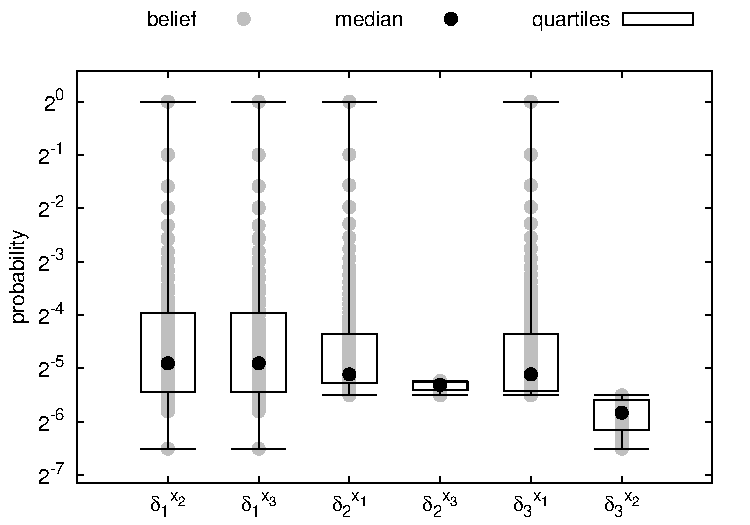
\includegraphics[width=8.5cm]{figures/beliefs_run_example.pdf} \\
\caption{Running example $Q_1$; plot of max beliefs}
\label{fig:run-example}
\end{figure}

\begin{figure}[t]
\scriptsize
\centering
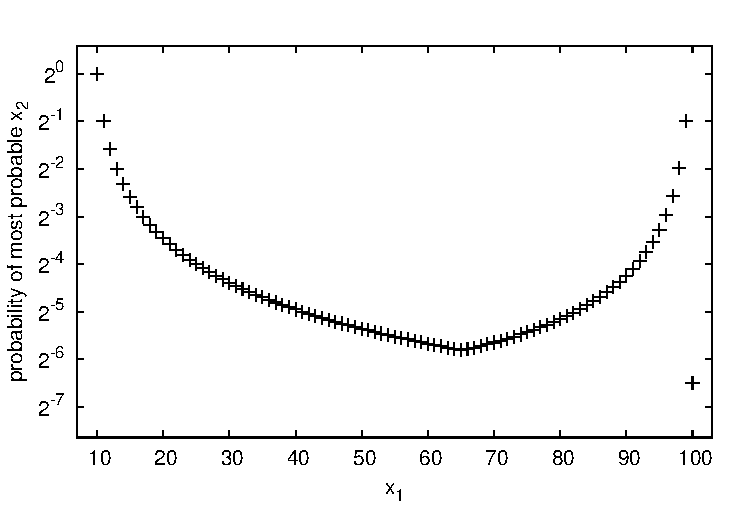
\includegraphics[width=8.5cm]{figures/beliefs_run_col1.pdf} \\
\caption{Running example $Q_1$; $ \delta_1^{x_2} $; plot of $ P_1 $'s
max belief about $ x_2 $ vs. values of $ x_1 $}
\label{fig:run-example-col1}
\end{figure}

\paragraph*{``Am I the richest?'' example ($Q_1$).}
Consider the running example query $ Q_1 $. If all the principals were
to evaluate threshold policies to determine the safety of $ Q_1 $,
they would reason about possible revised beliefs of the participants,
where the possibilities vary in their valuation of those participants'
secret values, as is described in \sref{sec:belief-set}. If the
principals perform this policy check via SMC, they would do so for
only one of those possible valuations.

We can better understand the relationship between the two approaches
by looking at the range of possible revised beliefs achievable. For
some secret values, a principal might learn little; for others, they
might learn a lot. \mwh{Use a small example to say what you mean here?
   For example, you could use the simple ``less than'' example from
   the introduction} We measure this range in terms of the probability
of the most probable secret in a principal's belief, for a given
valuation of their own secret.

\fref{fig:run-example} demonstrates the situation for the running
example, query $ Q_1 $, starting from the initial belief $\delta $
uniformly distributing values in $ 10 \leq x_1, x_2, x_3 \leq
100$. There are 6 relationships considered, for each principal $ P_i
$, during their policy decision to allow $ P_j $, with $ j \neq i $,
to see the query output, they would compute $ P_j $'s potential belief
about $ x_i $ (labeled $ \delta_j^{x_i} $ in the figures). These
beliefs depend on $ x_j $; the figure shows the potential belief for
every possible $ x_j $, the median belief achievable over them as well
as the 1st and 3rd quartiles, showing the range of $ P_j $'s likely
knowledge.\footnote{It is important to mention that our probabilities
are sometimes not exact due to the limitations of the implementation
used for the analysis. The true probabilities, however, cannot be
larger than those presented here. This imprecision is the reason why
belief sets representing $ P_2 $ and $ P_3 $'s beliefs about each
other, or about $ P_1 $, in \fref{fig:run-example} appear different,
though in actuality they are the same.}

\fref{fig:run-example-col1} focuses on the first column of \fref{fig:run-example}, $ \delta_1^{x_2} $, showing $ P_1 $'s
knowledge about $ x_2 $, depending on the value of $ x_1 $. At the very
top, the most $ P_1 $ could learn is when $ x_1 = 10 $ and the query
returns $ true $, meaning $ P_1 $ was the richest, with the smallest
amount of wealth. This lets $ P_1 $ conclude that $ x_2 = 10 $ and $
x_3 = 10 $. $ P_1 $'s potential knowledge of $ x_2 $ decreases as $
P_1 $'s wealth grows, up to $ x_1 = 65 $. At 65, if $ P_1 $ is the
richest, it is able to narrow $ x_2 $ down to 56 values (10 through
65). Starting with $ x_1 = 66 $, however, $ P_1 $ can learn more if
the query returns $ false $, stating that either $ P_2 $ or $ P_3 $ is
richer than $ P_1 $. Further increase in $ x_1 $, increases its
potential knowledge of $ x_2 $, culminating at $ x_1 = 99 $ which lets
$ P_1 $ conclude that $ x_2 = 100 $ with a probability close to $ 0.5
$. At $ x_1 = 100 $, the query can only return $ true $, hence $ P_1 $
learns nothing, keeping its knowledge of $ x_2 $ unchanged at $ 1/91
$. \mwh{Have you said anywhere that you are using belief distributions
  $\delta_1$ etc. from the earlier section?  You might be explicit
  about that if I'm right}

We see that for this query, the belief sets approach would
conservatively conclude that all participants could learn $ x_1 $
exactly, and that $ P_1 $ could learn $ x_2 $ and $ x_3 $ exactly. On
the other hand, it is impossible for $ P_2 $ and $ P_3 $ to learn each
other's values to any confidence.

The benefit of the SMC approach to policy enforcement is that it is
free from the overly conservative view of the belief sets approach. In
75\% (observing the upper extent of the quartile boxes) or more of the
situations, the actual beliefs of the participants do not exceed
probability of $ 2^{-4} \approx 0.06 $, which is comparable to the
$ \frac{1}{91} \approx 0.01 $ probability each agent started with. In
terms of utility, if the participants set their policy thresholds to
as little as 0.06, their policies would allow $ Q_1 $ in most
cases. The belief sets approach would reject $ Q_1 $ for all $t_i < 1$.

Not all queries are pathological for the belief sets approach. We next
look at a parameterized query that offers a security vs. utility tradeoff.

\begin{figure}[t]
\centering 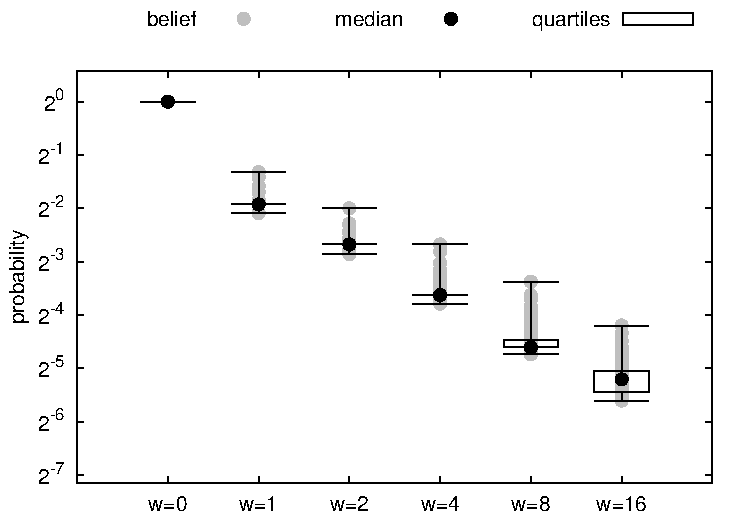
\includegraphics[width=8.5cm]{figures/beliefs_similar.pdf}
$$ \begin{array}{lcl}
similar_w & \defeq & \sassign{avg}{\frac{x_1+x_2+x_3}{3}} \\
&& \sifk\; \abs{x_1 - avg} \leq w \; \wedge \\
&& \quad   \abs{x_2 - avg} \leq w \; \wedge \\
&& \quad   \abs{x_3 - avg} \leq w \\
&& \quad \sthenk\;\sassign{out}{\strue} \\
&& \quad \selsek\; \sassign{out}{\sfalse}
\end{array} $$
\vspace*{-0.1in}
\caption{$ similar_{w} $ example; plot of max belief for a variety of
windows $ w $ sizes} \label{fig:similar}
\vspace*{-0.1in}
\end{figure}
\paragraph*{``Similar'' example} The query $ similar_w $, depicted at
the bottom of \fref{fig:similar}, determines
whether each principal's secret is within $ w $ of the
average. The choice of window size $ w $ determines how much the
principals can learn.\footnote{Note that the language described in
  \fref{fig-sem-nondet2-core} cannot
directly express this query due to the lack of the division and absolute
value operations. However, we can achieve the same effect by
multiplying all expressions by 3 and replacing the conditions on
absolute values by a pairs of upper and lower bounding conditions.}
The plot at the top of the figure shows the possible beliefs after evaluating $
similar_w $ with a variety of window values $ w $, with the initial
assumption that all values $ x_i $ are in uniformly distributed in $
1 \leq x_i \leq 100 $ (so each of the 100 possibilities has
probability $0.01$). The scenario
is thus completely symmetric in respect to the agents, hence only one
of the beliefs is shown in the figure.

When $ w = 0 $, the query can be completely revealing, as when it
returns true, all secrets are equal. Relaxing the window reduces how
much each agent can learn. At $ w = 2 $, each agent, in the worst
case, learns every other principal's secret with confidence of $ 0.25
$. This worst case already allows non-trivial threshold
policies. Going further, with the window set to $ 16 $, the query
becomes barely revealing, resulting in confidence never reaching over
$ 0.05 $, comparable to the initial $ 0.01 $. Further increase of $ w
$ can make the query even less revealing to the point of not releasing
any information at all, though of course also not providing any
utility.

\paragraph*{``Millionaires'' example.} The common motivating example
for SMC is a variant of $Q_1$ involving
a group of millionaires wishing to determine which of them is the
richest, without revealing their exact worth. The query $ richest_p $,
given at the bottom of \fref{fig:million},
accomplishes this goal, determining which of 3 participants is
(strictly) richer than the other two. An addition to this query has
been made to provide a means of injecting noise into its answers to
limit potential knowledge gain.

The output $ out = 0 $ designates that none of the three were strictly
richest. The query is concluded with a step that noises the
result. The assignment $ \sassign{out}{\mathit{uniform}\set{0,1,2,3}} $ is
shorthand notation for a series of $ \spifk $ statements, whose effect
is to set $ out $ to one of the $ 4 $ values, with uniform
probability. Thus given the parameter $ p $, this query will just
randomly return, with probability $ p $, one of the 4 possible
outputs.

\begin{figure}[t]
\centering
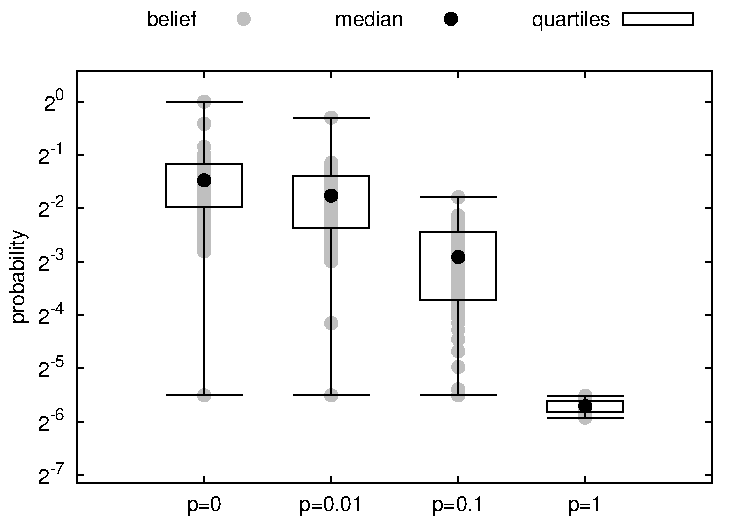
\includegraphics[width=8.5cm]{figures/beliefs_million.pdf}
$$ \begin{array}{lcl}
richest_p & \defeq & \sassign{out}{0} \\
&& \sifk\; x_1 > x_2 \; \wedge \; x_1 > x_3 \; \sthenk \; \sassign{out}{1} \\
&& \sifk\; x_2 > x_1 \; \wedge \; x_2 > x_3 \; \sthenk \; \sassign{out}{2} \\
&& \sifk\; x_3 > x_1 \; \wedge \; x_3 > x_2 \; \sthenk \; \sassign{out}{3} \\
&& \spifk\; p \; \sthenk \; \sassign{out}{uniform\set{0,1,2,3}}
\end{array} $$
\vspace*{-0.1in}
\caption{$ richest_{p} $ example; plot of max belief for a variety of
noising probabilities $ p $} \label{fig:million}
\end{figure}

A significant benefit of using probabilistic programming languages is
that the effect of non-determinism described using these probabilistic
statements is taken into account; we can determine exactly what a
rational agent would conclude from learning the output of such a
noised query.

\fref{fig:million} summarizes the beliefs of every agent assuming
initially each is equally likely to be worth between \$10 and
\$100. This scenario is also symmetric hence only the belief of one
agent about a single other agent is shown.

With $ p = 0 $, that is, no chance of random output, the query is
potentially fully revealing, but in most cases still keeping the
participants below $ 0.5 $ certainty. With a $ 0.01 $ chance of random
output, the worst case no longer results in absolute certainty, though
close to it. Randomizing the output with $ p = 0.1 $, keeps the
agents' certainty almost below $ 0.5 $ in the worst case.  Getting
closer to $ p = 1 $ the beliefs approach the initial ones. At $ p = 1
$ the query reveals nothing, though our approximate implementation
does produce some variation in the upper bound.

\section{Related Work}
Almost all prior work on SMC treats the function $f$ being computed by
the parties as given, and is unconcerned with the question of whether
the parties should agree to compute $f$ in the first place.  The only
exceptions we are aware of are two
papers~\cite{EC:DKMMN06,C:BeiNisOmr08} that consider SMC in
conjunction with \emph{differential
  privacy}~\cite{TCC:DMNS06,ICALP:Dwork06}.  Dwork et
al.~\cite{EC:DKMMN06} show that if $f$ is a differentially private
function, then the process of running an SMC protocol that
computes~$f$ is also differentially private (at least in a
computational sense). Beimel et al.~\cite{C:BeiNisOmr08} observe that
if the end goal is a distributed protocol that is differentially
private, then SMC may be overkill and more efficient alternatives may
be possible.

The security goal we are aiming for is incomparable with that of
differential privacy. \jnote{Right?}  Moreover, in contrast to
above-mentioned work, our determination of whether a function $f$ is
``safe'' to compute will explicitly depend on the parties' actual
inputs as well as any (known or assumed) prior knowledge that parties
have about each others' inputs.

\mwh{might steal some comments from related work in CSF paper.}

\section{Conclusions}

In this paper we have presented two methods that apply
\emph{knowledge-based security policies} to the problem of determining
whether participating in a secure multiparty computation could
unsafely reveal too much about a participant's secret input.  Ours are
the first techniques that consider the actual secrets and prior
knowledge of participants (potentially gained from previous SMC's)
when making this determination, making our approach more permissive
(in accepting more functions), and potentially safer, than techniques
that disregard this information.  Experiments with the two methods
show that the \emph{SMC belief tracking} method is the more permissive
of the two, but it remains to be seen whether this method can be
implemented efficiently.

%\vspace*{.1in}
%\begin{small}
%\paragraph*{Acknowledgments}
%This research was sponsored by the U.S. Army Research Laboratory and
%the U.K. Ministry of Defence and was accomplished under Agreement
%Number W911NF-06-3-0001. The views and conclusions contained in this
%document are those of the author(s) and should not be interpreted as
%representing the official policies, either expressed or implied, of
%the U.S. Army Research Laboratory, the U.S. Government, the
%U.K. Ministry of Defence or the U.K. Government. The U.S. and
%U.K. Governments are authorized to reproduce and distribute reprints
%for Government purposes notwithstanding any copyright notation hereon.
%\end{small}

\bibliographystyle{plain}
\bibliography{conf,abbrev_short,biblio}

\end{document}


% \section{OLD; may want to merge in}

% Facebook and other services derive a large part of their usefulness
% from the sharing of their user's often private information. Users
% maintain relationships with friends and enjoy a personal online
% experience while Facebook generates revenue from likewise
% trailed advertisements. Users, unfortunately, have little control over
% their private data and how it is used. One proposal to deal with the
% issue is to enable users to store and administer their data
% personally, providing an interface for others to query their
% data. Such an approach has some advantages:

% \begin{itemize}
% \item{} \textbf{Trust}. Handling your data yourself has
% firstly the simple benefit that you no longer need to trust other
% parties to handle your data in a safe manner.
% \item{} \textbf{Non-commitment}. A query interface approach has a
% distinct advantage over pre-privitizing \pxm{not sure if correct term}
% techniques; the future use cases of the data need not be known.
% \end{itemize}

% As an example of the benefit of non-commitment, consider a user
% protecting their birthday. They might decide it is safe for anyone to
% know their birthday to within 7 possible days and such might release
% the week of their birthday instead of the entire secret. This might
% serve its purpose for an advertiser wishing to offer them a special
% birthday offer in the general date but would prevent another party
% from determining whether they were born on a weekend (for whatever
% reason). On the other hand, if the user instead reduced their data to
% either born on weekend or not, it would also satisfy their privacy
% needs, but would make the data useful to the second party, but not the
% first.

% Non-commitment lets the user answer either of the two queries, and
% even both if he is sure the issuers of the two queries are not
% colluding.

% \subsection{Query safety}

% The problem, then, becomes how to determine whether a query is safe to
% answer.

% Various approaches exist to statically measure the information release
% potential of a query \pxm{cite some}, with the intent of rejecting
% queries deemed to release too much. Such approaches, however, need to
% analyze a sequence of queries as one, thereby limiting the usefulness
% of non-commitment. Furthermore the static measures often compute the
% expectation of information release, given a distribution of the user's
% secrets. This has the unfortunate consequence of a user with unlikely
% secret values concluding a query is safe to answer in expectation but
% actually is very revealing in their specific case.

% More dynamic approaches \cite{mardziel11belief} directly model what
% potential adversaries know about a users secret data and how this
% knowledge changes as a result to queries. A policy which asserts a
% limit to adversary's knowledge can then be maintained. Such a
% knowledge limit serves to protect the user, not just
% the \emph{expected} user. The queries in such an approach need not be
% known ahead of time.

% Knowledge in the dynamic approach is modeled as a probability
% distribution over the user's data. Adversary's learning is then
% Bayesian revision. The computational techniques to maintain this model
% centrally involve probabilistic program evaluation, a lifting of
% standard state-to-state evaluation to a distribution-to-distribution
% evaluation. This and other details including policy checking are
% computationally expensive. As a result approximations, sound in terms
% of the policy, are employed.

% \subsection{Multiple secrets}

% The case in which only one party is protecting their secrets, though
% applicable to many situations, does not admit other relevant
% situations. In the case of military coalition information sharing, the
% coalition partners often need coordinate actions without revealing too
% much about their forces. Determining the closest unit to a location on
% the battlefield, for example, might be useful and safe in terms of
% some knowledge-based policy but revealing the location of the
% coalition forces to each coalition might be deemed unsafe.

% The multi-secret case brings forth some challenges, however. Firstly,
% in order to accurately model what an agents knows about a user, the
% user needs to take into account the values of the agent's secret data,
% data the user does not know. Secondly, the evaluation of a query
% involving multiple agents' secrets cannot be easily performed, given
% the lack of data. Fortunately, techniques of secure multi-party are
% designed to exactly solve the second challenge and can also help to
% alleviate the first.

% Secure multi-party computation allows multiple parties to evaluate a
% function over their private data without revealing this private data,
% other than what can be inferred from the output of the function. The
% critical for situations with potentially mistrusting parties that
% cannot rely (or trust) a third party to perform this task.

% What exactly the parties can infer about each others' secrets is not
% of concern but can be problematic. In some situations knowing the
% query output goes a large way in determining the/some input to beyond
% a safe amount. Query analysis can thus be beneficial for checking
% queries are safe to securely compute.

% \pxm{probably more about secure computation}

% Secure computation not only allows one to compute the function
% securely, but also allows the parties to model each other's beliefs,
% taking into account the secret values they do not know, while
% asserting knowledge limits. This can be accomplished by performing
% knowledge-based policy enforcement and query evaluation as a secure
% computation.

% \pxm{\textbf{Outline}}

% \pxm{
%         Overview of belief tracking, CSF paper. Perhaps an
% example that could be easily extended to more than 1 party having a
% secret later.
%             Reason about what can be inferred/implied from the output
%             of a query. Restricted to a single individual holding the
%             private data.
%         Overview of SMC
%             Multiple parties having secrets and evaluating a query.
%             Parties learned nothing except what is implied by output,
%             but what exactly is implied?
%         Reconcile issues from both belief tracking and SMC by
%         combining them.
%             can evaluate queries involving secrets of more than 1
%             party
%             can reason about what query outputs actually reveal
%             as long as we can
%                 perform belief tracking in a secure way
%                 make sure there are no unmodeled information leaks
% }

% \section{Background}

% \subsection{Belief modeling}

% The core idea in knowledge based security enforcement is the modeling
% of the knowledge of a potential adversary and how this knowledge
% changes as a result from learning outputs to queries over one's
% secret data. We briefly summarize the idea here, further details can
% be found in \cite{clarkson09quantifying}.

% In the two party setting, we have two agents $ a_1, a_2 $ with $ a_1 $
% protecting a secret $ x_1 $. Also, $ a_2 $ has some, potentially
% incorrect, belief about $ x_1 $ defined as a probability distribution
% $ \delta $ over the possible values $ x_1 $ can have. In general, such
% probability distributions can be defined over program states and in
% this case we assume program states containing only a single variable,
% $ x_1 $.

% $$ \states = \set{\sigma : \vars \ra \Integer} $$
% $$ \dists = \set{\delta : \states \ra \Real} $$

% A probabilistic semantics is defined, so that given a query $ f $, and
% a belief $ \delta $, the distribution over program states after
% evaluating $ f $ is $ f(\delta) $. Furthermore, if $ output $ is a
% variable, intended to model the output to agent $ a_2 $ of the query
% and $ x $ is a possible value of this variable, then
% $ \dcond{f(\delta)}{\paren{output = x}} $ is the revised
% distribution, over secret values, given the observation that $ output
% = x $. If we let $ x = f(x_1)(output) $, that is, the output of the
% query evaluated on the actual secret $ x_1 $, then we can model the
% change in the belief given output of $ f $. Such a revised belief can
% then be used as the prior belief for a future query.

% It is shown in \cite{clarkson09quantifying} that the probabilistic
% semantics and revision exactly model the changing belief of an
% adversary as he learns outputs of the queries, assuming no other
% channel of information flow exists, and the adversary is rational and
% has unbounded computational power.

% \begin{theorem}[Theorem 1 of \cite{clarkson09quantifying}]
% A rational, computationally unbounded agent, having belief $ \delta $
% about $ x_1 $, updates his belief to $ \delta' $ after learning output
% of a query $ f $, with no other channels, where $ \delta' $ is
% $ \dcond{f(\delta)}{\paren{output = x}} $.
% \end{theorem}

% The model can easily be extended to multiple agents querying the
% data by merely considering several beliefs $ \delta_i $, one for each
% such agent. As long as the agents do not share information then this
% would model would accurately represent their beliefs about the user's
% secret. In the case of collusion, however, this is no longer the case.

% In the situation of collusion, the user might choose to assume a set
% of agents share information, and thus represent their knowledge as a
% single distribution, being revised when any of them received a new
% query output. This approach, however, can break the claim that the
% distributions accurately represent the agents' belies. If the agents
% are not actually colluding, their attributed knowledge could be in
% some measure more accurate. This might itself not be a problem if one
% is interested in enforcing some policy over the knowledge (see next
% section).

% There are some situations in which learning the output of a query can
% reduce the agents certainty about the user's secret. Queries that
% involve probabilistic chance, that happen to take an unlikely outcome,
% serve to \emph{confuse} instead of clarify. In the setting of
% collusion, if the user assumes collusion which actually does not
% occur, he might attribute \emph{less} knowledge to a colluding agent
% than they actual have.

% Consider a simple query that checks whether the user is male but that
% also has a $ 1/5 $ chance of flipping its result.

% is-maybe-male$(gender) \defeq $
% \begin{algorithmic}
% \IF{gender == ``male''}
% \STATE {output := true}
% \ELSE
% \STATE {output := false}
% \ENDIF
% \IF{random() $ \leq 0.2 $}
% \STATE {output := not output}
% \ENDIF
% \end{algorithmic}

% Assume the initial belief of the querier is uniform in gender,
% $ \delta(\text{gender = male}) = \delta(\text{gender = female}) = 0.5
% $. The effect of the query on $ \delta $ is another distribution
% $ \delta' = \text{is-maybe-male}(\delta) $ with the following probabilities.
% \begin{align*}
% \delta'(\text{gender = male, output = true}) &= 0.4 \\
% \delta'(\text{gender = male, output = false}) &= 0.1 \\
% \delta'(\text{gender = female, output = true}) &= 0.1 \\
% \delta'(\text{gender = female, output = false}) &= 0.4
% \end{align*}
% Now, even when gender of the user is actually male, the function can
% let output be false, and in this situation, the revised belief
% $ \dcond{\delta'}{\paren{output=false}} = \delta'' $, we have a
% $ \delta'' $ which has less certainty in the actual gender of the user
% than the original $ \delta $:
% \begin{align*}
% \delta''(\text{gender = male}) &= 0.2 \\
% \delta''(\text{gender = female}) &= 0.8
% \end{align*}
% One potential solution to this is to notify all
% colluding agents of all the query outputs (and queries) of the agents
% involved. It would be in their rational interest to take this
% information into account when reasoning about the user's secret.

% \subsection{Policy enforcement}

% One can naturally use the belief model to enforce a knowledge-based
% policy, making sure that the knowledge of the adversary doesn't grow
% beyond a certain bound.

% A variety of bounds can be defined to limit the knowledge. A natural
% one is to bound the probability of the actual secret to be below a
% certain threshold, $ \delta(x_1 = v) \leq t $, where $ v $ is the
% actual value of $ x_1 $, and $ t $ is some real in $ [0,1] $. The
% user can then only answer queries as long as the revised belief would
% satisfy this predicate. It is shown in \cite{mardziel11belief} that
% this kind of policy has danger of leaking information from rejection
% as the policy depends on the actual secret.

% The user can make sure the predicate always hold by instead checking
% the revised belief over all secrets and all possible query outputs,
% which itself includes the actual secret and the actual query output
% respectively. Such a predicate is function of not the revised belief,
% but the probabilistically interpreted prior belief $ f(\delta) $. We will
% designate this or any other policy on this belief as $ P_1 $.

% A query interface would then be a simple procedure $ P_f $ of the secret $ x_1
% $ and the belief $ \delta $ about this secret:

% $ P_f(x_1, \delta) \defeq $
% \begin{algorithmic}[1]
% \STATE $ \underline{\delta} := f(\delta) $
% \IF{not $ P_1(\underline{\delta}) $}
% \RETURN{$\delta$ to $a_1$, reject to $a_2$}
% \ELSE
% \STATE $x := f(x_1)(output) $
% \RETURN{$\underline{\delta} | x$ to $a_1$, $x$ to $a_2$}
% \ENDIF
% \end{algorithmic}

% We assume above that agent $ a_1 $ is the user holding the secret
% while $ a_2 $ is the querier. The output to $ a_1 $ is merely meant to
% convey the potentially updated belief.

% %in-range$(p, r) \defeq $
% %\begin{algorithmic}
% %\IF{dist $\paren{p, a_1} \leq r $}
% %\STATE $output := true$
% %\ELSE
% %\STATE $output := false$
% %\ENDIF
% %\end{algorithmic}

% There are two important issues in knowledge-based policy
% enforcement; the issue of computational cost, and the issue of the
% initial belief.

% \pxm{\textbf{Outline}}

% \pxm{
%         Some details about the CSF paper, beliefs, probabilistic
%         evaluation, revision, policy definition.
%             Note approximation and domains usable with their cost.
%         Some details about SMC, perhaps just stating that a circuit
%         output is evaluated without (computational) revelation of the
%         inputs.
%             Note the computational expense of the approach as well as
%         limitation (finite data, others?)
%             Mention fastgc and potential benefits (or otherwise why
%         are we using it?)
% }

% \section{Methodology}

% Let us first consider the case of modeling the knowledge two parties,
% each having a secret. Here we will assume that queries can access both
% secrets, and have separate outputs to the two agents. We will
% designate the outputs with $ output_i $. We will also write $
% output_{1,2} $ to designate an output to both agents. An example of a
% two-agent query is the closer$_p$ query which checks which agent's secret
% value is closer to some given point $ p $.

% closer$_p(x_1, x_2) \defeq $
% \begin{algorithmic}
% \IF {$ dist\paren{\var{p}, \var{x_1}} \leq
% dist\paren{\var{p}, \var{x_2}} $}
% \STATE $ output_{1,2} := 1 $
% \ELSE
% \STATE $ output_{1,2} := 2 $
% \ENDIF
% \end{algorithmic}

% Ignoring the issue of how the agents can actually evaluate this query,
% we can consider the beliefs of the agents and how they would change,
% assuming they only learn the query outputs. Let us say $ a_1 $ and $
% a_2 $ have beliefs $ \delta^1_2 $ and $ \delta^2_1 $ about $ x_2 $ and
% $ x_1 $ respectively. We can model each agent's reasoning
% separately. Agent $ a_1 $ knows $ x_1 $, hence his view of the query
% is $ f(x_1, \delta^1_2) $, that is, $ x_1 $ is a constant, not a
% distribution, whereas the second argument is $ a_1 $'s belief about $
% x_2 $. If the query output to $ a_1 $ is $ o_1 $, then $ a_1 $'s belief after
% learning $ o_1 $ is $ \dcond{f(x_1, \delta^1_2)}{\paren{output_1 = o_1}}
% $. Similarly $ a_2 $'s belief will be
% $ \dcond{f(\delta^2_1,x_2)}{\paren{output_2 = o_2}} $.

% \begin{theorem} Assume rational and computationally unbounded agents $ a_1, a_2 $, initially hold beliefs
% $ \delta^1_2, \delta^2_1 $, respectively, about each other's secrets,
% $ x_1, x_2 $. Assuming no other channels, if the agents learn their
% respective outputs $ o_1, o_2 $ of $ f(x_1, x_2) $, their knowledge
% will become $ \underline{\delta^1_2}, \underline{\delta^2_1} $,
% respectively, where
% $$ \underline{\delta^1_2} = \dcond{f(x_1, \delta^1_2)}{\paren{output_1
% = o_1}} $$
% $$ \underline{\delta^2_1} = \dcond{f(\delta^2_1, x_2)}{\paren{output_2
% = o_2}} $$
% \end{theorem}

% \pxm{some sort of argument for a proof}

% \subsection{More than two parties}

% The extension of the system to more than two parties is in some ways
% straightforward but also contains several wrinkles. Since queries can
% involve more than 1 agent's secrets, we must handle beliefs agents
% have about more than 1 other agent. This allows us to handle
% dependencies that can be created in the beliefs. Furthermore, when
% considering policy checks more than two agents must be guaranteed
% secrecy and integrity of the belief and the task of producing the
% initial distributions is made more complex. Finally, the issue of
% collusion must be considered.

% It will be now convenient to view functions $ f $ as taking a state
% argument and producing a state output. If we write $ f(x_1=v_1,
% x_2=v_2) $ we assume the function evaluates from the state in which $
% x_1 = v_1 $ and $ x_2 = v_2 $. Also, probabilistic evaluation of $ f $
% will be written similarly as $ f(x_1 = v_1, \delta) $ where variable $
% x_1 $ is assumed to be a constant, and the rest of the variables are
% represented by the distribution $ \delta $.

\subsection{Dependency}

Consider a simple query that checks whether the secret values of two
agents are equal, and reports this to a third agent:

same$_{i,j,k}(x_1, x_2, s_3) \defeq $
\begin{algorithmic}
\IF {$s_i = s_j$}
\STATE $output_k = true $
\ELSE
\STATE $output_k = false $
\ENDIF
\end{algorithmic}

If $ a_3 $ learns that same$_{1,2,3}$ output $ true $, he can form a
correlation between $ a_1 $ and $ a_2 $'s secret values without
actually knowing what that value is. If subsequently $ a_3 $ learns
that same$_{2,3,3}$ was $ true $ as well, he would be able to infer
the value of $ x_1 $, even though $ x_1 $ was not involved in the
second query at all. The policy of $ a_1 $, therefore, must be
considered when evaluating same$_{2,3,3}$.

Given the ability of agents to form dependencies, we need to model
beliefs of an agent over the secret values of all other
agents.

\begin{theorem} Assume a set $ A $ of $ n $ rational and computationally unbounded agents $
a_i $ holding secrets $ s_i $ respectively, initially believe
$ \delta^i $ about agents $ (A - \set{a_i}) $'s secrets.  Assuming no
other channels, if the agents learn their respective outputs $ o_i $
of $ f(x_1=v_1, ..., s_N=v_N) $, their knowledge will become
$ \underline{\delta^i} $ where
$$ \underline{\delta^i} = \dcond{f(s_i=v_i, \delta^i)}{\paren{output_i
= o_i}} $$
\end{theorem}

\subsection{Policy}
In the simplest terms, the two-party knowledge-based security
enforcement is merely two instances of one-party enforcement,
performed in a secure manner so as to provide the means for the agents
to actual model the knowledge change occurring.

Let $ s_i $ be the secret of agent $ a_i $ and let $ \delta^i_j $ be
the distribution agent $ i $ has to model agent $ j $'s knowledge
about agent $ i $'s secrets. Also let $ f $ be the query and $ P_i $
be the policy agent $ i $ wants to enforce. We can thus extend the
single-secret case as follows.

$ P_f(x_1, x_2, \delta^2_1, \delta^1_2) \defeq $
\begin{algorithmic}[1]
\STATE $ \underline{\delta^2_1} := f(\delta^2_1,x_2) $
\IF{not $ P_1(\underline{\delta^2_1}) $}
\RETURN{$\delta^2_1$ to $a_1$, reject to $a_2$}
\ELSE
\STATE $x := f(x_1, x_2)(output_1) $
\RETURN{$\underline{\delta^2_1} | x$ to $a_1$, $x$ to $a_2$}
\ENDIF
\STATE $ \underline{\delta^1_2} := f(x_1,\delta^1_2) $
\STATE ...
\end{algorithmic}

The procedure first produces the distribution $ \underline{\delta^2_1}
$, using probabilistic interpretation on the distribution $ \delta^2_1
$, the belief $ a_2 $ has about $ x_1 $. If $ a_1 $'s policy $ P_1 $
checks out on this distribution, the actual query output, $ x $ is
computed and the revised belief $ \underline{\delta^2_1} | \var{x} $
and output $ x $ is returned to agents $ a_1 $ and $ a_2 $
respectively. On the other hand if the policy check fails, $ a_1 $
gets the original distribution and $ a_2 $ gets $ \mathit{reject}
$. The procedure is then repeated enforcing $ a_2 $'s policy.

There is an issue that complicates the matters, however. If $ a_1 $
learns the revised belief or learns its policy rejected a query, he
can potentially infer something about $ x_2 $, as there is a clear
channel of information flow from $ x_2 $ to both the revised belief
and the rejection/non-rejection branches of the algorithm, via
$ \underline{\delta^2_1} $. We must thus ensure the agents cannot
learn anything about the modeled beliefs, but at the same time we must
ensure the agents can trust that their policies are evaluated on
accurate beliefs.

\pxm{an example here of knowing revised, or knowing reject/non-reject
leaks information}


\subsection{Policies for more than two parties}

As the same$_{1,2,3}$ example demonstrated, every agent has interest
in the knowledge bounds of attributed any other agent's belief about
them and therefore the integrity of the belief's representation.

\subsection{Belief maintenance}

An agent cannot learn the belief other agents have about its secret,
but must make sure this belief is accurate. Let us say $ n $ agents
need to provide mutual secrecy and integrity of a belief represented
as an $m$-bit value, we define three functions with the following
properties.
\newcommand{\zon}{\set{0,1}^{n}}
\newcommand{\zom}{\set{0,1}^{m}}
\newcommand{\tf}{\set{true,false}}

\begin{itemize}
\item{encode $: \zom \times \paren{\zom}^n \ra \zom $} - Given a value $ v
$, $ n $ bit vectors $ r_i $ each of length $ m $, the function produces
the value $ v' $ such that agent $ a_i $ knowing only $ r_i $
and $ v' $ cannot reconstruct $ v $, but the agents together can
reconstruct $ v $ and be assured of its integrity (below).

\item{reconstruct $: \zom \times \paren{\zom}^{n} \ra \zom $} - Given value $ v'
$ and $ n $ bit vectors $ r_i $ recovers value $ v $ produced using encode.

\item{verify $: \paren{\zom}^{n} \ra \tf$} -
Given values $ v_i $, determines whether they agree as to the original
source value, a means with which agents can be sure the value was not
tampered with.

\end{itemize}

An implementation of the above requirements can be constructed using
xor operations.
\[
\begin{array}{l}
\text{encode}(v, r_1, ..., r_n) \defeq (v \oplus r_1 \oplus ... \oplus r_n) \\
\\[-1ex]
\text{reconstruct} \defeq \text{encode} \\
\\[-1ex]
\text{verify}(v_1, ..., v_n) \defeq \\
\;\;\; v_1 = v_2 = ... = v_n
\end{array}
\]

\pxm{not sure if the function signatures are right for whatever crypto
scheme exists out there to ensure this}

\newcommand{\adelta}{\sim\delta}

The two-party belief tracking scheme now requires the agents to
provide additional inputs, namely the random bits $ r_i $ for each
distribution. The agents will also maintain each distribution as two
values, the encoded distribution, and a portion of the random bits
used to produce it, each portion held by one of the agents. We will
write $ \adelta $ to designate the combination of the encoded values,
the random bits used to encode it, and a set of new random bits for
future re-encoding. Then $ a_i(\adelta) $ will designate the pair $
v_i, r_i $ where $ v_i $ is the encoded value held by and provided by
agent $ a_i $ and $ r_i $ are that agent's contributing random
bits. Also, $ v_i(\adelta) $, $ r_i(\adelta) $, $ r'_i(\adelta) $ will denote the
values, random bits, and fresh random bits contributed by agent $ a_i
$. The fresh random bits are required to re-encode distributions and
using old random bits would allow agents to detect policy rejections
from the observation that the belief has not changed.

$ P_f(x_1, x_2, \adelta^2_1, \adelta^1_2) \defeq $
\begin{algorithmic}[1]
\IF{not verify($v_1(\adelta^2_1), v_2(\adelta^2_1)$)}
\RETURN{error to everyone}
\ELSE
\STATE $ \delta^2_1 := $ reconstruct($v_1(\adelta^2_1),
r_1(\adelta^2_1), r_2(\adelta^2_1)$)
\STATE $ \underline{\delta^2_1} := f(\delta^2_1,x_2) $
\IF{not $ P_1(\underline{\delta^2_1}) $}
\STATE $ \adelta^2_1 := $ encode($\delta^2_1, r'_1(\adelta^2_1), r'_2(\adelta^2_1)$)
\RETURN{$a_1(\adelta^2_1)$ to $a_1$, ($a_2(\adelta^2_1)$, reject) to $a_2$}
\ELSE
\STATE $x := f(x_1, x_2)(output_1) $
\STATE $\underline{\adelta^2_1} := $ encode( $\underline{\delta^2_1} | x,
r'_1(\adelta^2_1), r'_2(\adelta^2_1)$ )
\RETURN{$a_1(\underline{\adelta^2_1})$ to $a_1$,
($a_2(\underline{\adelta^2_1}), x$) to $a_2$}
\ENDIF
\ENDIF
\IF{not verify($v_1(\adelta^1_2), v_2(\adelta^1_2)$)}
\STATE ...
\ENDIF
\end{algorithmic}

Note that in this scheme, an agent doesn't know whether its policy is
rejecting queries. One might think that once an agent starts to get
rejections, he will refuse to participate further and thereby
suggesting the fact he is being rejected to the other agent. We note,
however, that refusing further participation can only hurt the agent
refusing to participate, namely the information flow we are preventing
by not letting$ a_1 $ know that $ a_2 $ is getting rejected is from $
a_2 $'s secret to $ a_1 $. Hence if $ a_2 $ refuses to participate and
$ a_1 $ determines that this is most likely because $ a_2 $ is getting
rejected, $ a_1 $ might be able to infer something about $ x_2 $.

\subsubsection{Initial distributions}

\pxm{Mention something about how the two parties initially create the
$ \adelta $ from what they believe each other knows about them.}

\pxm{In case they think the other party knows more than they actually
do, we can say that we will reveal the initial distributions to
everyone, so thus they will know at least that much.}

$S(\delta^2_1,r_{1,1},r_{1,2},\delta^1_2, r_{2,1}, r_{2,2}) \defeq $
\begin{algorithmic}[1]
\STATE $ \adelta^2_1 := $ encode($\delta^2_1, r_{1,1}, r_{1,2}$)
\RETURN{$a_1(\adelta^2_1)$ to $a_1$, $a_2(\adelta^2_1)$ to $ a_2 $}
\STATE $ \adelta^1_2 := $ ...
\end{algorithmic}

\subsection{Belief handling}

\pxm{Describe how to use crypto to spread the distributions among n
agents so they are all sure of its integrity and secrecy}

\subsection{Initial distributions}

\pxm{Each agent probably knows best what is known about them in the
world, hence they would be best ones to produce a belief about
them. But we need to have joint distributions. In the case of no
initial dependence, we can take the distribution cross products,
otherwise each agent will have to decide how others view them IN TERMS
of other agents, that is, joint distributions.}

\subsection{Collusion}

\pxm{Describe a way to let a distribution be evaluated with more than
1 party's actual secret if an agent beliefs some are colluding.}

\pxm{To handle confusion from unlikely query results, we can just say
that if we assume two parties are colluding, then we will always give
them each other's outputs. This creates a challenge in deciding an
agreement between all agents as to who is colluding.}

\pxm{The agreement procedure above would probably involve some
invocation of SMC.}

\pxm{\textbf{Outline}}

\pxm{
        Mention once more the issues of both belief tracking and SMC
        from the introduction. This time go into more detail as to why
        there are issues.
            Explore troubles one would have trying to solve belief
        tracking in multiparty case and how without knowing the other
        party’s secret, we have a hard time figuring out what they
        might belief.
                Potential solutions to this being infeasible
        computationally.
                But we can use SMC to perform belief tracking without
        having to know the other party’s secret.
        The main approach: belief tracking over SMC.
            Make a claim as to the outcomes of the system (without
        fully defining it): assuming participant’s initial beliefs are
        captured correctly, assuming they bring in no other knowledge
        than the one from interaction with our system, and assuming
        the agents are rational bayesian agents, then at all times, we
        maintain their actual belief. Additionally, we can perform
        policy decision over such beliefs in a manner that preserves
        the policy.
                How to write the above in a more concise manner?
        Details how to accomplish the claim to complete the section.
        Cannot learn the belief, but can enforce it.
            Crypto means of shared maintenance of belief.
        Policy issues in the multiparty (more than 2 case)
            Issues of dependence.
                if a.x == b.x then output true to c
            Solution assuming everyone is colluding. Mention confusion
        as a problem.
            Solution assuming not, larger belief complexity, but
        allows modeling of dependence in belief between secrets of
        different agents.
        Complexity
            Mention once more normal belief tracking benchmarks over
        various domains as in the background.
            Mention inefficiency of SMC.
            Speculate as to the combined complexity (how?)
            Why bother with this as there are really no other viable
        options to compare to?
}

\section{Results}
\pxm{
        Implementation
            some fastgc details and benefits
            mention how belief tracking was implemented
            probabilistic query evaluation including policy checking
            and various checks need to be implemented as a circuit
                no interpreter, the evaluator is specific to query
            used
                belief and policy reused from each query evaluation,
            but the circuit is remade for each query
                circuit implementation of (box?) domain with finite
            components (a parameter)
            secure but oblivious maintenance of belief
            secure policy evaluation
            a lot of details which I have no idea about right now
        Some benchmarks on various queries and/or query
            sequences. Also provide a measure of max-belief using a
            more complex domain in a non-SMC simulation to show what
            is lost using the box domain.
            Who-is-richer? (millionaires)
            Who-is-closer? This would be a good one for a sequence of
            queries with different location to test closeness to.
}

\section{Related Work}
\cite{mardziel11belief}
\cite{huang11efficient}
\pxm{
        Mention current work on SMC and future potential of ever
        increasing performance?
        The usual story of how belief tracking can be better than more
        static QIF measures, copy from CSF paper.
        The usual comparison of differential privacy and its
        non-applicability to this case. Perhaps speculate to
        applications in which differential privacy would be applicable
        and conjecture whether a similar approach can be taken.
}

\section{Conclusions}
\pxm{
        Mention the main claim once more.
        Mention the benchmarks.
        Mention potential future work
            code splitting into potentially SMC-evaled components
            query hiding by code as data in SMC
}

% LocalWords:  CSF SMC unmodeled

